\documentclass{article}
\usepackage{arxiv}

\captionsetup[figure]{labelfont=it,textfont={it}}


\title{Detecting confounder and center bias in machine learning models}



\author{
  Tamas~Spisak \\
  Institute for Diagnostic and Interventional Radiology and Neuroradiology \\
  University Hospital Essen\\
  Hufelandstrasse 55, 45147 Essen \\
  \texttt{tamas.spisak@uk-essen.de} \\
  %% examples of more authors
  %% \AND
  %% Coauthor \\
  %% Affiliation \\
  %% Address \\
  %% \texttt{email} \\
  %% \And
  %% Coauthor \\
  %% Affiliation \\
  %% Address \\
  %% \texttt{email} \\
  %% \And
  %% Coauthor \\
  %% Affiliation \\
  %% Address \\
  %% \texttt{email} \\
}

\begin{document}
\maketitle

%TC:ignore
\begin{abstract} % 150 words
The lack of rigorous non-parametric statistical tests for confounder effects significantly hampers the development of robust, valid and generalizable predictive models in many fields of research.

Here I propose the \emph{partial} and \emph{full confounder tests}, that build on a recently established theoretical framework for permutation-based conditional independence testing and, for a given confounder variable, probe the null hypotheses of \emph{unconfounded} and \emph{fully confounded models}, respectively.

The tests provide a strict control for Type I errors and high statistical power, even for non-linear and non-normal dependencies typical in machine learning.
Applying the proposed tests on models trained on functional brain connectivity data from the Human Connectome Project and the Autism Brain Imaging Data Exchange dataset reveals confounders that were previously partly unreported and found to be hard to correct for with state-of-the-art confound mitigation approaches.

The package \emph{mlconfound}\footnote{\href{https://mlconfound.readthedocs.io}{https://mlconfound.readthedocs.io}} can aid the assessment and improvement of the generalizability and neurobiological validity of predictive models and, thereby, foster the development of clinically useful machine learning biomarkers.
\end{abstract}
%TC:endignore


% keywords can be removed
\keywords{machine learning, predictive modelling, confounder test, conditional independence, conditional permutation}

%%%%%%%%%%%%%%%%%%%%%%%%%%%%%%%%%%%%%%%%%%%%%%%%%%%%%%%%%%%%%%%%%%%%%%%%%%%
\section{Introduction}

Predictive modelling has recently become increasingly important in biomedical research and holds promise for delivering biomarkers that substantially impact clinical practice and public health\citep{kent2018personalized, spisak2020pain, walsh2021dome}. When evaluating the usefulness and applicability of such markers, predictive performance (i.e. prognostic/diagnostic value) is far from being the only important consideration. Biomedical validity (i.e. whether the model is driven by biomedically relevant signal) as well as generalizability and fairness across contexts and populations are crucial requirements for candidate biomarkers\citep{woo2017building, obermeyer2019dissecting, mehrabi2021survey}.

Spurious, out-of-interest associations between the predictor variables (features) and the prediction target - i.e the so-called confounder and collider biases\citep{prosperi2020causal} - can be detrimental to the model's biomedical validity and generalizability. Examples include models picking up on measurement artifacts (in-scanner head motion artifacts in magnetic resonance imaging-based predictive models of Alzheimer's\citep{rao2017predictive}, attention deficit hyperactivity disorder\citep{eloyan2012automated, couvy2016head} or Autism Spectrum Disorder (ASD)\citep{gotts2013perils, spisak2014voxel, spisak2019optimal}), demographic and psychometric variables (e.g models trained to predict intelligence\citep{ cole2012global, he2020deep} might provide a statistically significant predictive performance by picking up solely on age-related variance\citep{dubois2018distributed, lohmann2021predicting}), sampling bias and stochastic group differences (racially biased machine learning models\citep{ obermeyer2019dissecting, lwowski2021risk}), batch effects or, in multi-center studies, center-effects.

While various data cleaning methods might help in mitigating confounder bias\citep{rao2017predictive, dukart2011age, spisak2014voxel, abdulkadir2014reduction, rao2017predictive, johnson2007adjusting}, it is often unclear which variables should be considered as confounders during harmonization and such approaches hold risks of eliminating signal-of-interest\citep{wachinger2021detect}.

Powerful and robust statistical tests to quantify confounding effects in predictive models could substantially foster both the identification of confounders to correct for and the assessment of the effectiveness of various confound-mitigation approaches. Although confounder bias can be expressed in terms of conditional independence of the model predictions on the target and the confoudner variables, the proper evaluation of the conditional independence among these variables is challenging. Namely, even in the presence of a slight non-normality and/or non-linearity of the involved conditional distributions, the partial correlation analogs of bivariate non-parametric correlations (like the partial Spearman correlation) are not valid measures of conditional independence. Although warnings about this issue were given from early on\citep{korn1984ranges}, and received a fair amount of attention recently\citep{bergsma2010nonparametric, candes2016panning, peters2016causal,  shah2020hardness, berrett2020conditional}, the magnitude of the problem may not be fully appreciated in case of predictive model diagnostics, where non-normality and non-linearity of the model output can be frequently seen, as a consequence of e.g. feature-set characteristics and model regularization\citep{garcia2009study, kristensen2017whole}; see Supplementary Material \ref{sup:nomlinviol} for a simplistic example.

Alternative techniques for quantifying confoudner bias either fail to control type error (as  the known in the case of balanced permutations\cite{southworth2009properties, hemerik2018exact}, used in\cite{chaibub2019permutation}), or do not aim at all to do so\cite{ferrari2020measuring, wachinger2021detect}. 
Moreover, without some modifications, they are applicable for either only numeric\cite{wachinger2021detect} or only categorical variables\citep{chaibub2019permutation, ferrari2020measuring} and involve re-fitting the model\citep{chaibub2019permutation, ferrari2020measuring}, which might not be feasible for models with high a computational cost (e.g. with nested cross-validation). Some techniques\cite{wachinger2021detect}, furthermore, probe a null hypothesis (direct causation between the features and the prediction target) that is not applicable for for many kinds of data and models \footnote{For instance, causation between several psychological or clinical states and functional MRI activity/connectivity is obviously not \emph{direct}, as functional MRI itself is an \emph{indirect} measure of neural activation. In such cases, the alternative hypothesis of this test might be true in absence of any real confounder. }.

This work aims to construct a test of confounder bias which (i) can be applied post-hoc, without re-fitting the model (i.e. requires only the target variable, the confoudner and the model predictions), (ii) guarantees valid type-I error control even if the involved conditional distributions are non-normal and/or non-linear, (iii) is applicable for classification and prediction problems, both with numerical and categorical confounders.

% todo: RO and CI: classification, KC: regression

%In this paper, I formulate the 'confounder problem' as a special case of conditional independence testing\citep{dawid1979conditional}. This allows relating the problem to the seminal work of\cite{shah2020hardness}, who showed that, without placing some assumptions on the joint distribution of the involved variables, establishing a conditional independence test with a valid type I error control and non-trivial power is effectively impossible ('no free lunch' theorem). 
%As an important consequence, methods like partial correlation - and even its non-parametric variety - will fail if the corresponding conditional distributions are non-normal or if non-linear relationships are involved (see e.g.\citep{korn1984ranges} or Fig. \ref{fig:sim-h0-demo} in this paper), as commonly seen in machine learning.

%To overcome these limitations, I extend the permutation-based conditional independence framework of\cite{berrett2020conditional} with a generalized additive model based conditional distribution estimation, which allows avoiding to place any assumptions about the most problematic variable, the prediction output. 
%The framework allows constructing two tests: the \emph{full confounder test} probes whether the model's predictive performance can be attributed exclusively to the confounder and the \emph{partial confounder test} investigates whether the model utilizes any confounder-variance in the predictions, when controlled for the target variable.
%Both tests require only the target variable, the model predictions and the putative confounder as input, thus, they can be performed with a negligible extra computational cost (re-fitting the model is not required).
%The robustness of the type I error control and the statistical power of both tests are evaluated with simulated data (assuming non-normality and non-linearity).

%The usefulness of the proposed tests in detecting various types of confounder bias is demonstrated in two typical research scenarios (a regression and a classification problem) where confounder effects are known to harm building biomedically valid predictive models. 
%First, functional connectivity data from the Human Connectome Project (HCP)\citep{van2013wu} is used to build predictive models of fluid intelligence and to test for the previously discussed confounding effect of age\citep{ dubois2018distributed, lohmann2021predicting} and,  additionally, the - somewhat underdiscussed - batch-like effect of acquisition date of the data within the course of the data acquisition process.
%Second, functional connectivity data from the ABIDE\citep{di2014autism} database is used to investigate the potential motion- and center-bias\cite{gotts2013perils, spisak2014voxel, spisak2019optimal} when training models that aim to predict ASD diagnosis.

\section{Results}

% fig: overview
\begin{figure}[!b]
  \centering
  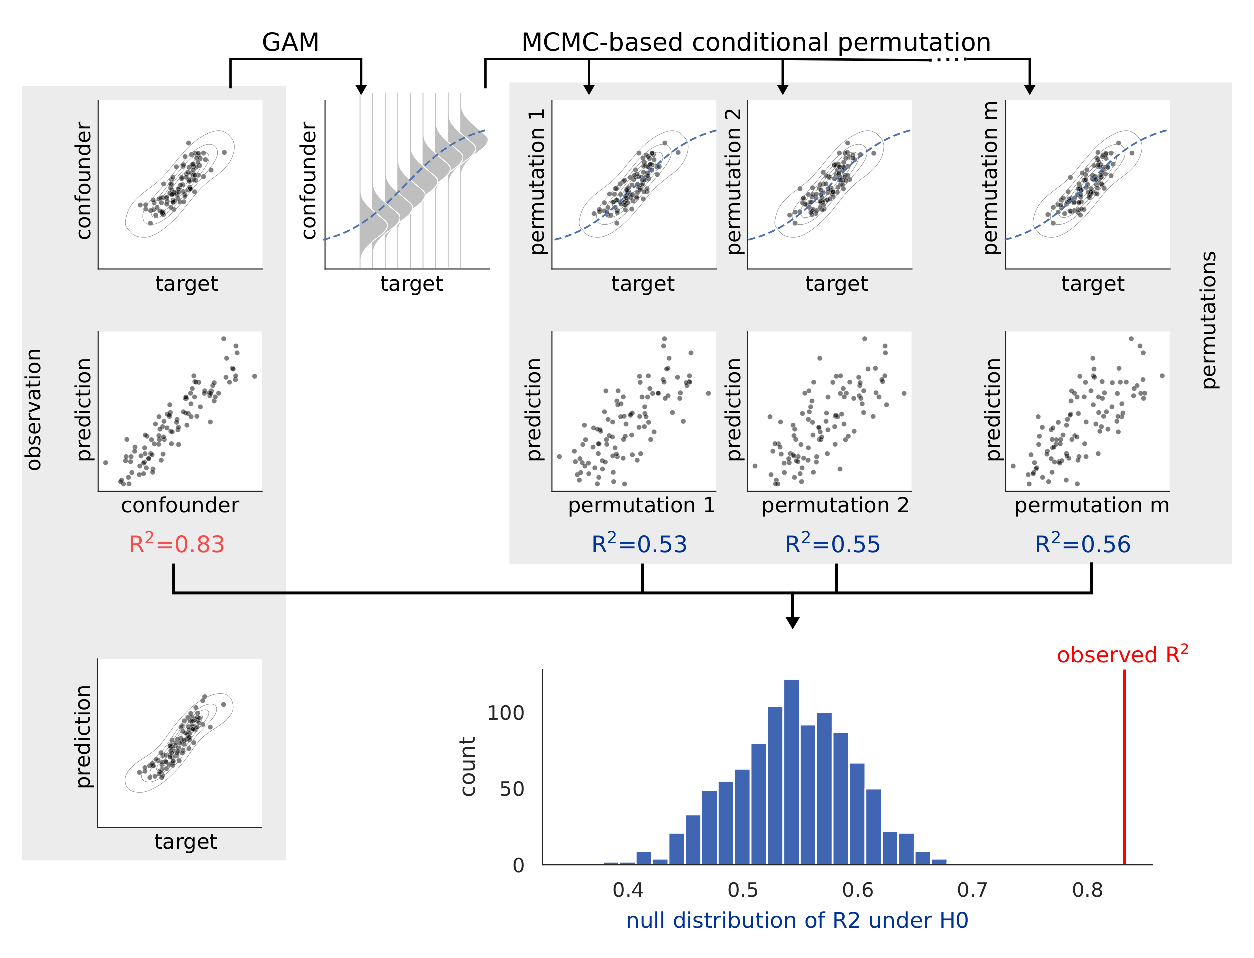
\includegraphics[width=0.75\paperwidth]{fig/overview.eps}
  \caption{\textbf{Overview of the proposed partial confoudner test}. \\
    The partial confoudner test models the conditional distribution of the confounder, given the target variable, with a generalized additive model (GAM). The parallel-pairwise Markov-chain Monte-Carlo sampler draws permutations of the confounder variable that comply with the GAM-based conditional distribution (permutation 1, 2, ..., m). The test statistic (coefficient of determination, $R^2$) is then computed between the model predictions and the original, as well as the permuted confoudner variables. The original and the permuted test statistics construct the p-value as the ratio of permuted test statistics more extreme than the original. Figure source code available as jupyter notebook: \href{https://github.com/pni-lab/mlconfound-manuscript/blob/main/simulated/overview-fig.ipynb}{https://github.com/pni-lab/mlconfound-manuscript/blob/main/simulated/overview-fig.ipynb}
  }
  \label{fig:overview}
\end{figure}

%%%%%%%%%%%%%%%%%%%%%%%%%%%%%%%%%%%%%%%%%%%%%%%%%%%%%%%%%%%%%%%%%%%%%%%%%%%

\subsection{The partial and full confoudner tests}


%fig:sim-h0-demo
\begin{figure}[!b]
  \centering
  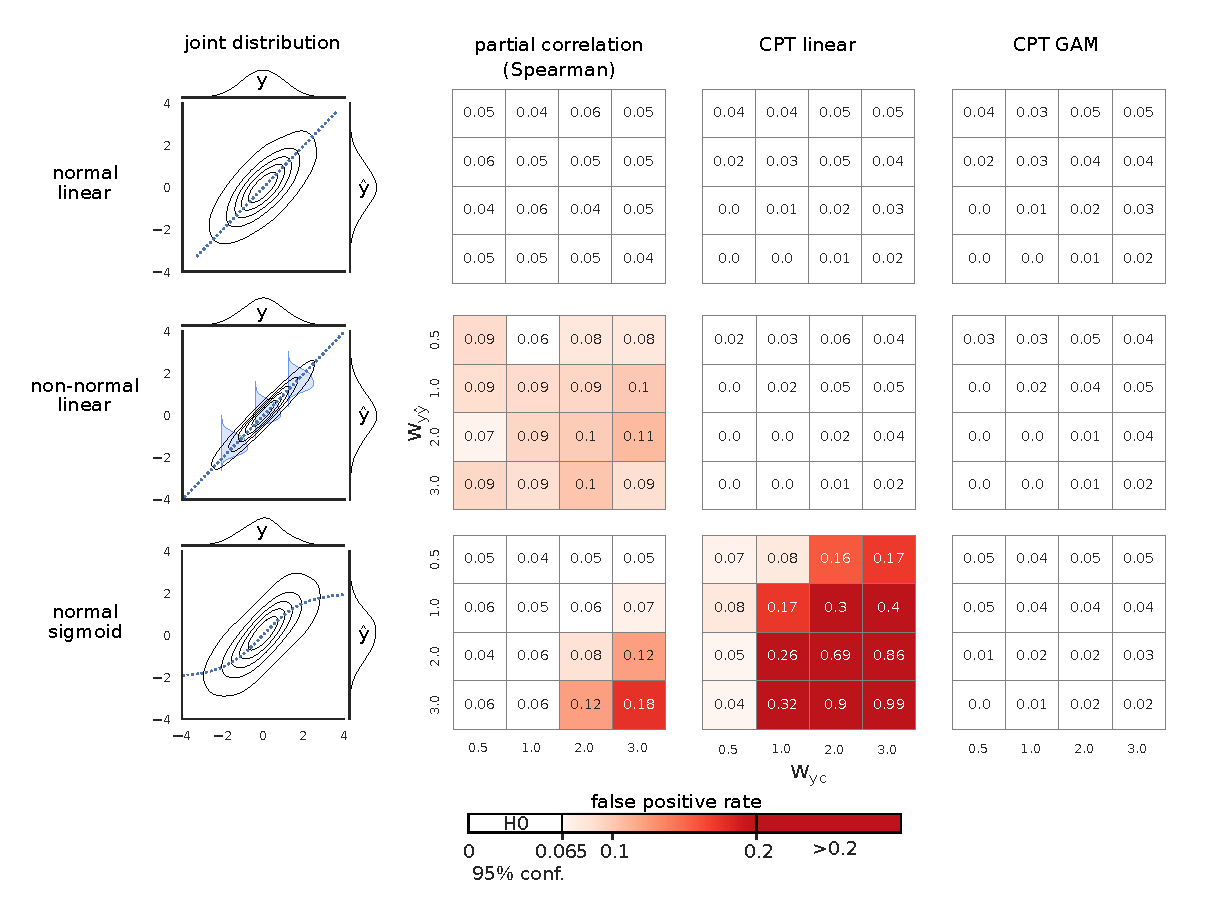
\includegraphics[width=0.75\paperwidth]{fig/sim_h0_demo.eps}
  \caption{\textbf{Type I error control of partial Spearman correlation, linear and GAM-based conditional permutation test}. \\
  Type I error control was investigated in three example cases: normal conditional distribution with linear dependency (first row), slightly non-normal conditional distribution with linear dependency (second row) and normal conditional distribution with non-normal (sigmoid) dependency (third row). Non-normal conditional distribution on the second plot is illustrated with blue density diagrams (kurtosis: -0.8, skewness: -0.1) and dependency of the mean is depicted with blue dotted lines an all plots. False positive rates for the three investigated tests is shown in heatmaps, with darker red meaning higher values. The upper limit for the binomial confidence interval corresponding to $alpha=0.05$ is 0.065. Values below this threshold indicate a valid type I error control and colored white.
  }
  \label{fig:sim-h0-demo}
\end{figure}

The idea of conditional independence provides a straightforward framework for assessing the confounder bias in predictive models. However, handling the non-normal and/or non-linear conditional dependence often seen in predictive models\citep{garcia2009study, kristensen2017whole} poses a great challenge.
In fact, as recently shown by Shah and colleagues\cite{shah2020hardness} in their 'no free lunch' theorem, it is effectively impossible to establish a fully non-parametric conditional independence test with a valid type I error control and non-trivial power. In practice, this means that all candidate tests, that assume normality and/or linearity of the joint distribution, will necessarily fail to properly control for Type I errors in many realistic predictive modelling scenarios. For instance, a trivial candidate, partial Spearman correlation, exhibits inflated type I errors even with slight violations of normality and linearity, as clearly demonstrated with simulated data on Fig. \ref{fig:sim-h0-demo}.

As the most problematic from the three variables (target, prediction, confounder) is clearly the model prediction\citep{garcia2009study, kristensen2017whole}, a method being distribution-free only for this variable might already provide a sufficient robustness for predictive model diagnostics. Exactly this can be achieved with the combination of the novel framework of conditional permutation testing (CPT)\cite{berrett2020conditional} and the use of generalized additive (GAM)\citep{hastie1987generalized} or multinomial logistic model\cite{bennett1966multiple, jones1975proability}-based conditional distribution estimation. The proposed approach offers two novel tests for probing confounder bias: the \emph{full confounder test} probes whether the model's predictive performance can be attributed exclusively to the confounder and the \emph{partial confounder test} investigates whether the model utilizes any confounder-variance in the predictions, when controlled for the target variable.
These tests place no assumptions on the conditional distributions of the model predictions, ensuring valid model diagnostics even in cases of non-normally and non-linearly dependent predictions.

The inner workings of the \emph{partial confoudner test} is summarized on Fig. \ref{fig:overview}. In short, the test models the conditional distribution between the confounder and the target variable with a generalized additive model (GAM) - or with a multinomial logistic regression, in case of categorical confounder - and then uses a so-called parallel-pairwise Markov-chain Monte-Carlo sampler that draws permutations of the confounder, so that the permuted variables still comply with the GAM-based conditional distribution. The test statistic (coefficient of determination, $R^2$) is then computed between the model predictions and the original, as well as the permuted variables. The original and the permuted test statistics construct the p-value as the ratio of permuted test statistics more extreme than the original. The \emph{full confoudner test} works in an analogous way, with the difference that it creates permuted copies of the target variable, instead of the confoudner.

These tests can handle both numerical and categorical data and can be applied for any predictive model, without having to re-fit the model, that is, with a negligible extra computational cost.
The proposed \emph{partial} and \emph{full confoudner tests} have been implemented in the python package \emph{mlconfound}\footnote{\href{https://mlconfound.readthedocs.io}{https://mlconfound.readthedocs.io}}. 

\subsection{Simulations}

%fig:sim-normal
\begin{figure}[!b]
  \centering
  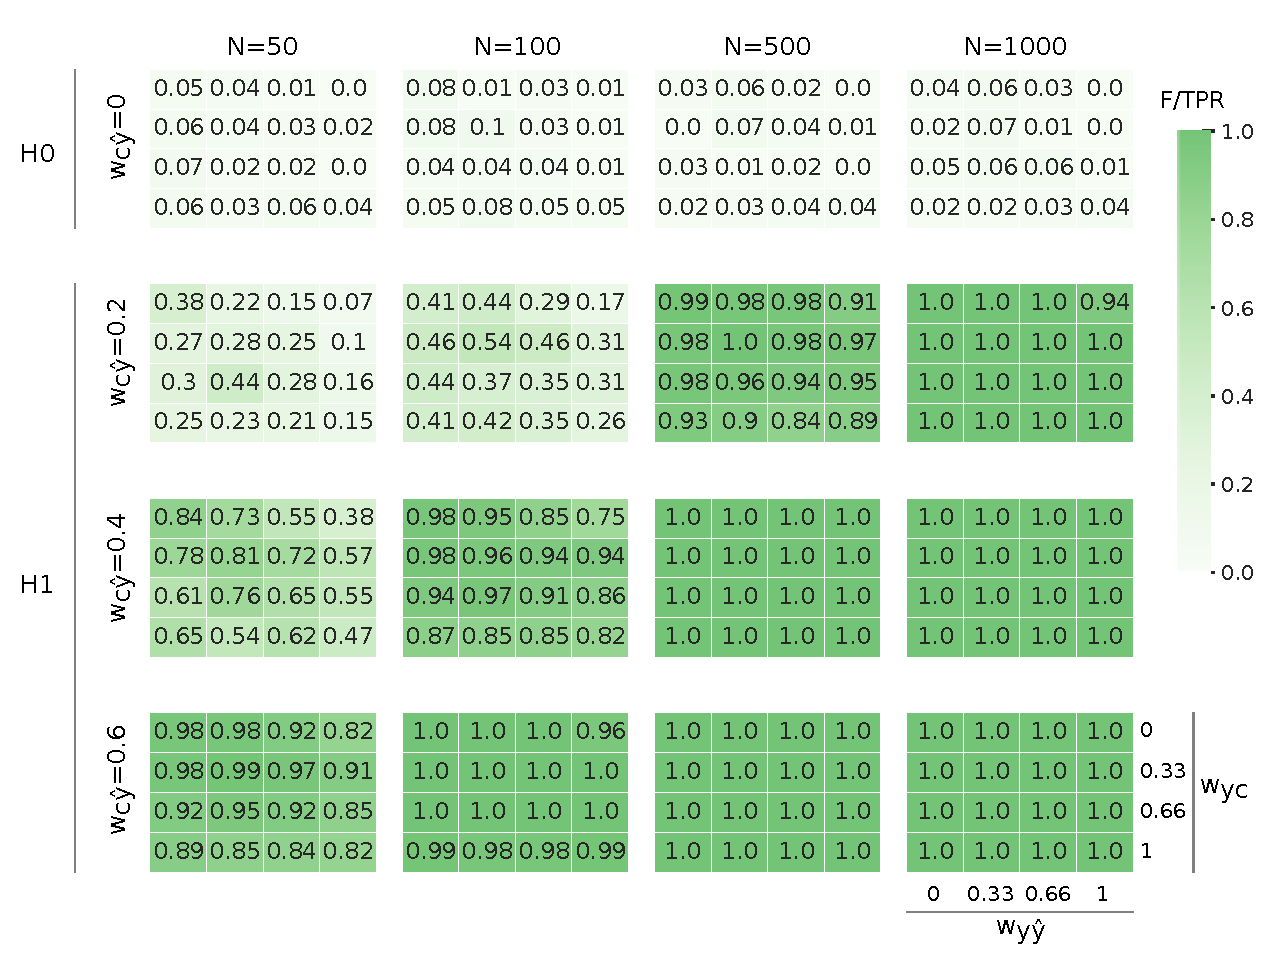
\includegraphics[width=0.75\paperwidth]{fig/sim_normal.eps}
  \caption{\textbf{Type I error control and power of the partial confoudner test based on simulations with normal conditional distribution and linear dependencies.} \\
  Heatmaps depict positive rates (ratio of p-values lower than 0.05, color coded as shown by the palette on the right) in various simulations settings (100 simulations per tile) with different simulation weights $w_{y\hat{y}}$ (horizontal axis on each heatmap), $w_{yc}$ (vertical axis on each heatmap), $w_{c\hat{y}}$ (rows) and for different sample sizes (N, columns). Weights 0.2, 0.33, 0.4, 0.6, 0.66, 1.0 can be assigned to the following approximate explained variance values: 4\%, 10\%, 12\%, 25\%, 30\%, 50\%. First row contains simulations under the null hypothesis (H0, no confounder effect), rows 2-4 represent simulations from the alternative hypothesis (H1, confounder bias).
  Positive rates for the simulations under the null and the alternative hypotheses can be interpreted as type I error rate and statistical power, respectively. The higher 95\% confidence limit for a positive rate of $alpha=0.05$ is 0.11 for each tile.
  }
  \label{fig:sim-normal}
\end{figure}

%fig:fig:sim-non-normal
\begin{figure}[!b]
  \centering

  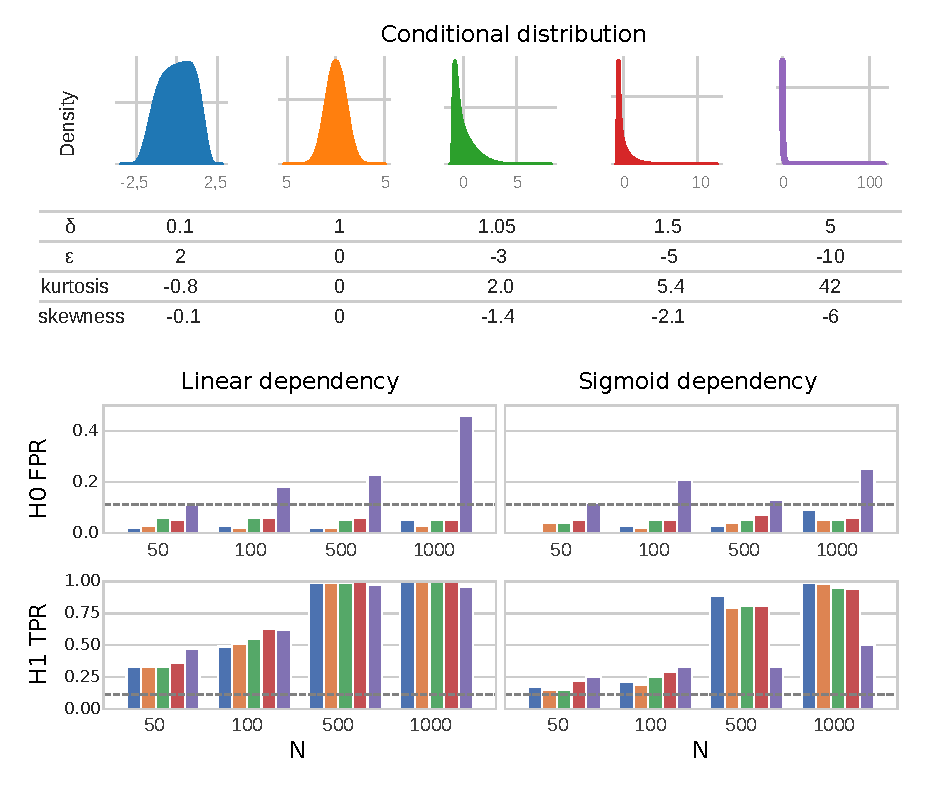
\includegraphics[width=0.5\paperwidth]{fig/sim_non-norm.eps}
  \caption{\textbf{Robustness of conditional permutation based confound testing to non-normality and non-linearity.} \\
  Simulations included variables with five different degrees of non-normality (top panel), as introduced with various $\delta$ and $\epsilon$ values of the \emph{sinh-arcsinh} transformation (yellow: normally distributed). Fisher's kurtosis and skewness is given for each distribution. False and true positive rates in the simulations under H0 and H1, respectively, for each investigated sample size (N), are depicted by barplots for both linear and sigmoid dependency structure. Upper 95\% binomial confidence limit corresponding to $alpha=0.05$ is shown with a vertical dashed line.}
  \label{fig:sim-non-normal}
\end{figure}

\subsubsection*{Type I error}

As suggested by theory (see \hyperref[sec:methods]{Methods} for details) and shown by the simulations with a wide range of settings, both of the proposed tests provide a valid Type I error control (Fig. \ref{fig:sim-normal}), even in case of non-linearity and non-normality (Figs. \ref{fig:sim-h0-demo} and \ref{fig:sim-non-normal}), except when non-normality is very extreme (purple distribution on Fig. \ref{fig:sim-non-normal}, kurtosis: 42, skewness: -6).

\subsubsection*{Power}

Estimates of statistical power for the partial confounder test (with normal and linear simulations, for  a wide range of parameters) are shown on Figure \ref{fig:sim-normal}. Notably, with sample sizes as large as 1000, a confounder contributing to only ~4\% to the variance of the predictions can already be robustly detected ($w_{c\hat{y}} = 0.2$) with a power of 94-100\%. With a sample size of 500, the same confounder bias is still detected with a power greater than 84\% in all of the simulation cases. A sample size of 100 requires a somewhat stronger bias with approximately 12\% of explained variance ($w_{c\hat{y}}=0.4$) for a robust detection, with a power of 75-98\%. Finally, even with a relatively low sample size of 50, the same amount of confounder variance is detected with a power of at least 50\%. If the confounder explains more than 25\% of variance, it is almost certainly detected even with the low sample size of $n \geq 50$.

Simulations with non-normal and non-linear dependencies has minimal effect on the power of the tests, except in case of extreme non-normality. (Fig. \ref{fig:sim-non-normal}).
Type I error and power was found to be highly similar in case of categorical variables and for the \emph{full} confounder test, as well (Supplementary Figures \ref{fig:sim-ccc-sig-partial}, \ref{fig:sim-bbb-lin-partial}, \ref{fig:sim-bbb-sig-partial}, \ref{fig:sim-ccc-sig-full}, \ref{fig:sim-bbb-lin-full} and \ref{fig:sim-bbb-sig-full}).


\subsection{Neuroimaging data}

To demonstrate the usefulness of the proposed tests in detecting various types of confounder-bias, they have been deployed in two typical research scenarios (a regression and a classification problem) where confounder effects are known to harm building biomedically valid predictive models. 

\subsubsection*{HCP dataset}

\begin{figure}[!b]
  \centering
  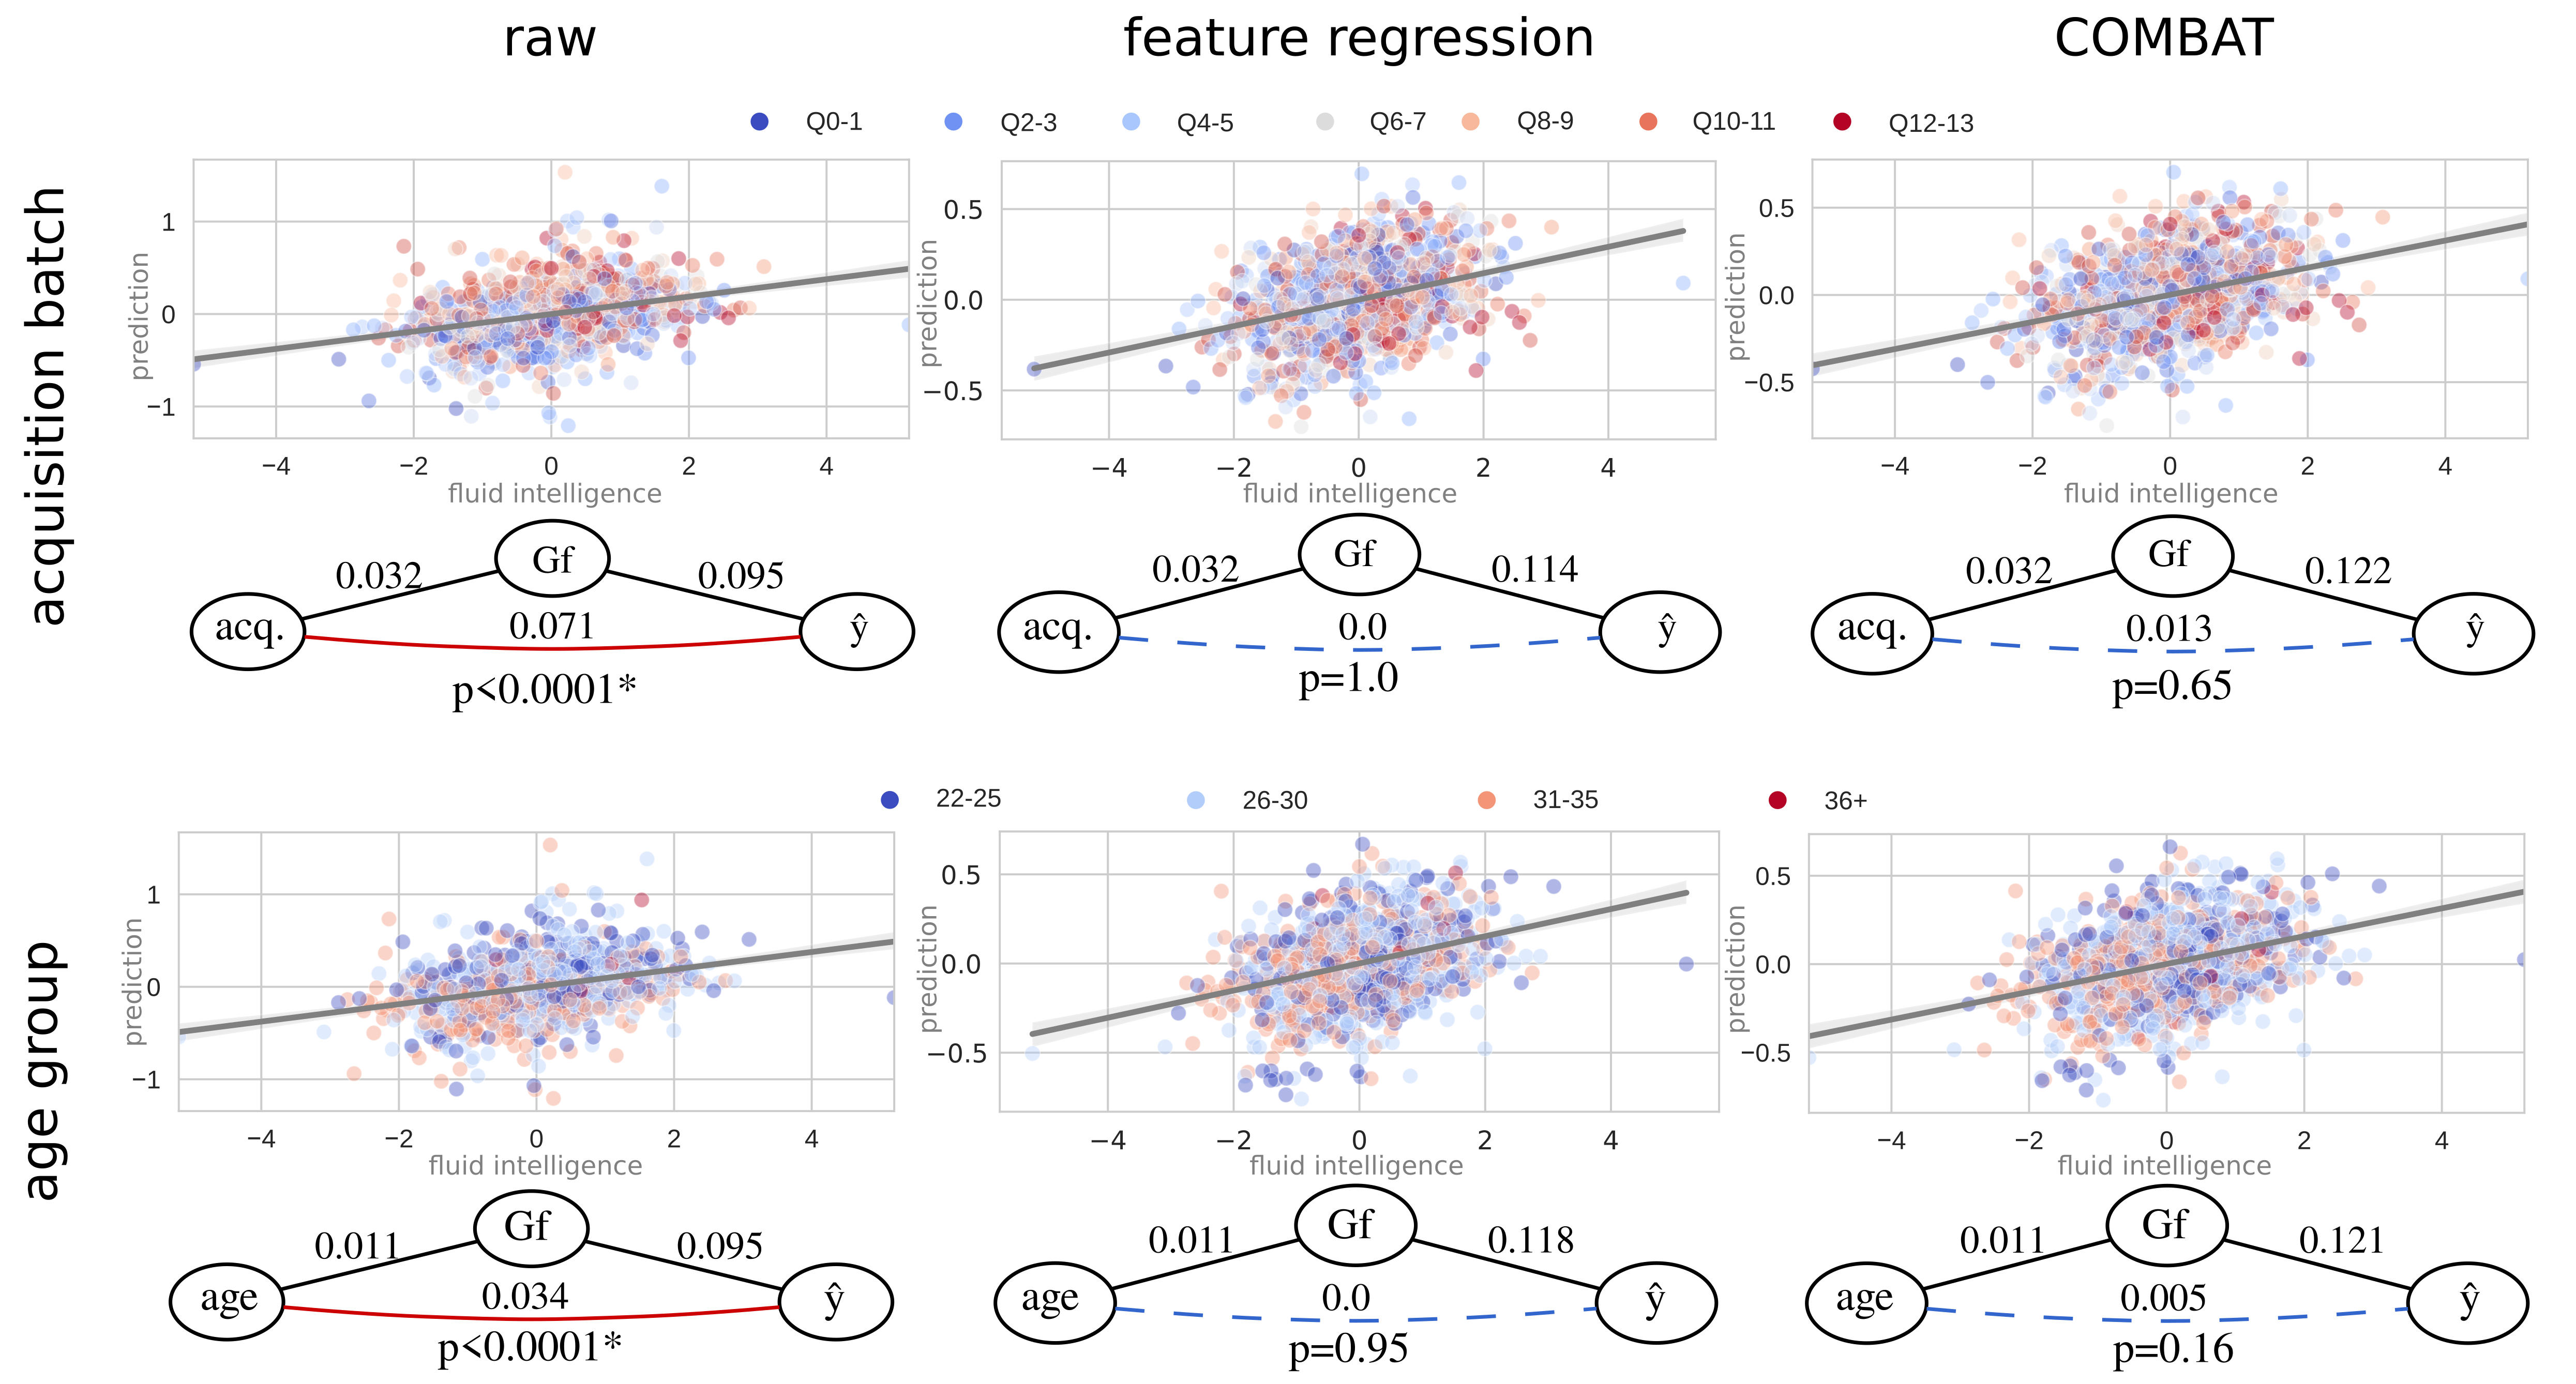
\includegraphics[width=0.75\paperwidth]{fig/fig_hcp.png}
  \caption{\textbf{Acquisition- and age-bias of fluid intelligence prediction in the HCP dataset.} \\
  Scatter plots and regression lines (with 95\% confidence intervals) show the association of the observed (horizontals axis) and predicted (vertical axis) fluid intelligence scores with various confound regression strategies. Color-coding of the confounder variables (top: acquisition batch, bottom: age group, as shown by the corresponding legends) reveals confounder-bias for both acquisition and age in the models trained on the raw data. This bias is robustly detected by the partial confounder test ($p<0.0001$) and seems to be effectively mitigated by both feature regression and COMBAT.
  Relation between the observed ($Gf$) and predicted ($\hat{y}$) IQ scores and the confounder variables is given on the graphs via $R^2 values$. Both confound mitigation techniques, but especially COMBAT, improves the predictive performance of the models.
  Solid red line between the confounder and the prediction means significant confounder bias, whereas blue dashed line denotes that confounder testing provided no evidence for bias. P-values are determined with the partial confound test. P-values of the 'full' confound test were all less then 0.0001, i.e. the confounders did not fully drive prediction for any of the models.
  }
  \label{fig:hcp}
\end{figure}

Functional connectivity data from the Human Connectome Project (HCP)\citep{van2013wu} was used to build predictive models of fluid intelligence and to test for the previously discussed confounding effect of age\citep{lohmann2021predicting, dubois2018distributed} and,  additionally, the - somewhat underdiscussed - batch-like effect of acquisition date of the data within the course of the data acquisition process.

Both acquisition batch and age group were statistically significantly associated with fluid intelligence ($R^2=0.032$ and $0.011$ and $p<0.001$ and $p=0.001$, respectively, see also Table \ref{tab:unconditional-pvals}). The model trained on the raw (unadjusted) connectivity features predicted fluid intelligence with a medium effect size ($R^2=0.095$, $p<0.001$).
The partial confounder test revealed that the model was significantly biased both by age group and acquisition batch (both $p<0.0001$, first column of Fig. \ref{fig:hcp}) with later phases of the acquisition and lower age being weakly-moderately ($R^2=0.071$ and $0.034$, respectively) associated to larger predicted values.

After applying confound mitigation approaches (feature regression or COMBAT) the partial confounder test did not provide evidence of confounder bias anymore ($p > 0.05$ for all; shown in the second and third columns of Fig. \ref{fig:hcp}), neither for acquisition batch nor for age. Both feature regression and COMBAT increased the predictive performance in the case of both confounders, with COMBAT providing best performances ($R^2=0.122$ and $0.121$ when applied to remove the effect of acquisition and age, respectively).

The full confounder test was highly significant ($p<0.0001$) for all models, indicating that neither of the models were exclusively driven by the confounds.

\subsubsection*{ABIDE dataset}

\begin{figure}[!b]
  \centering
  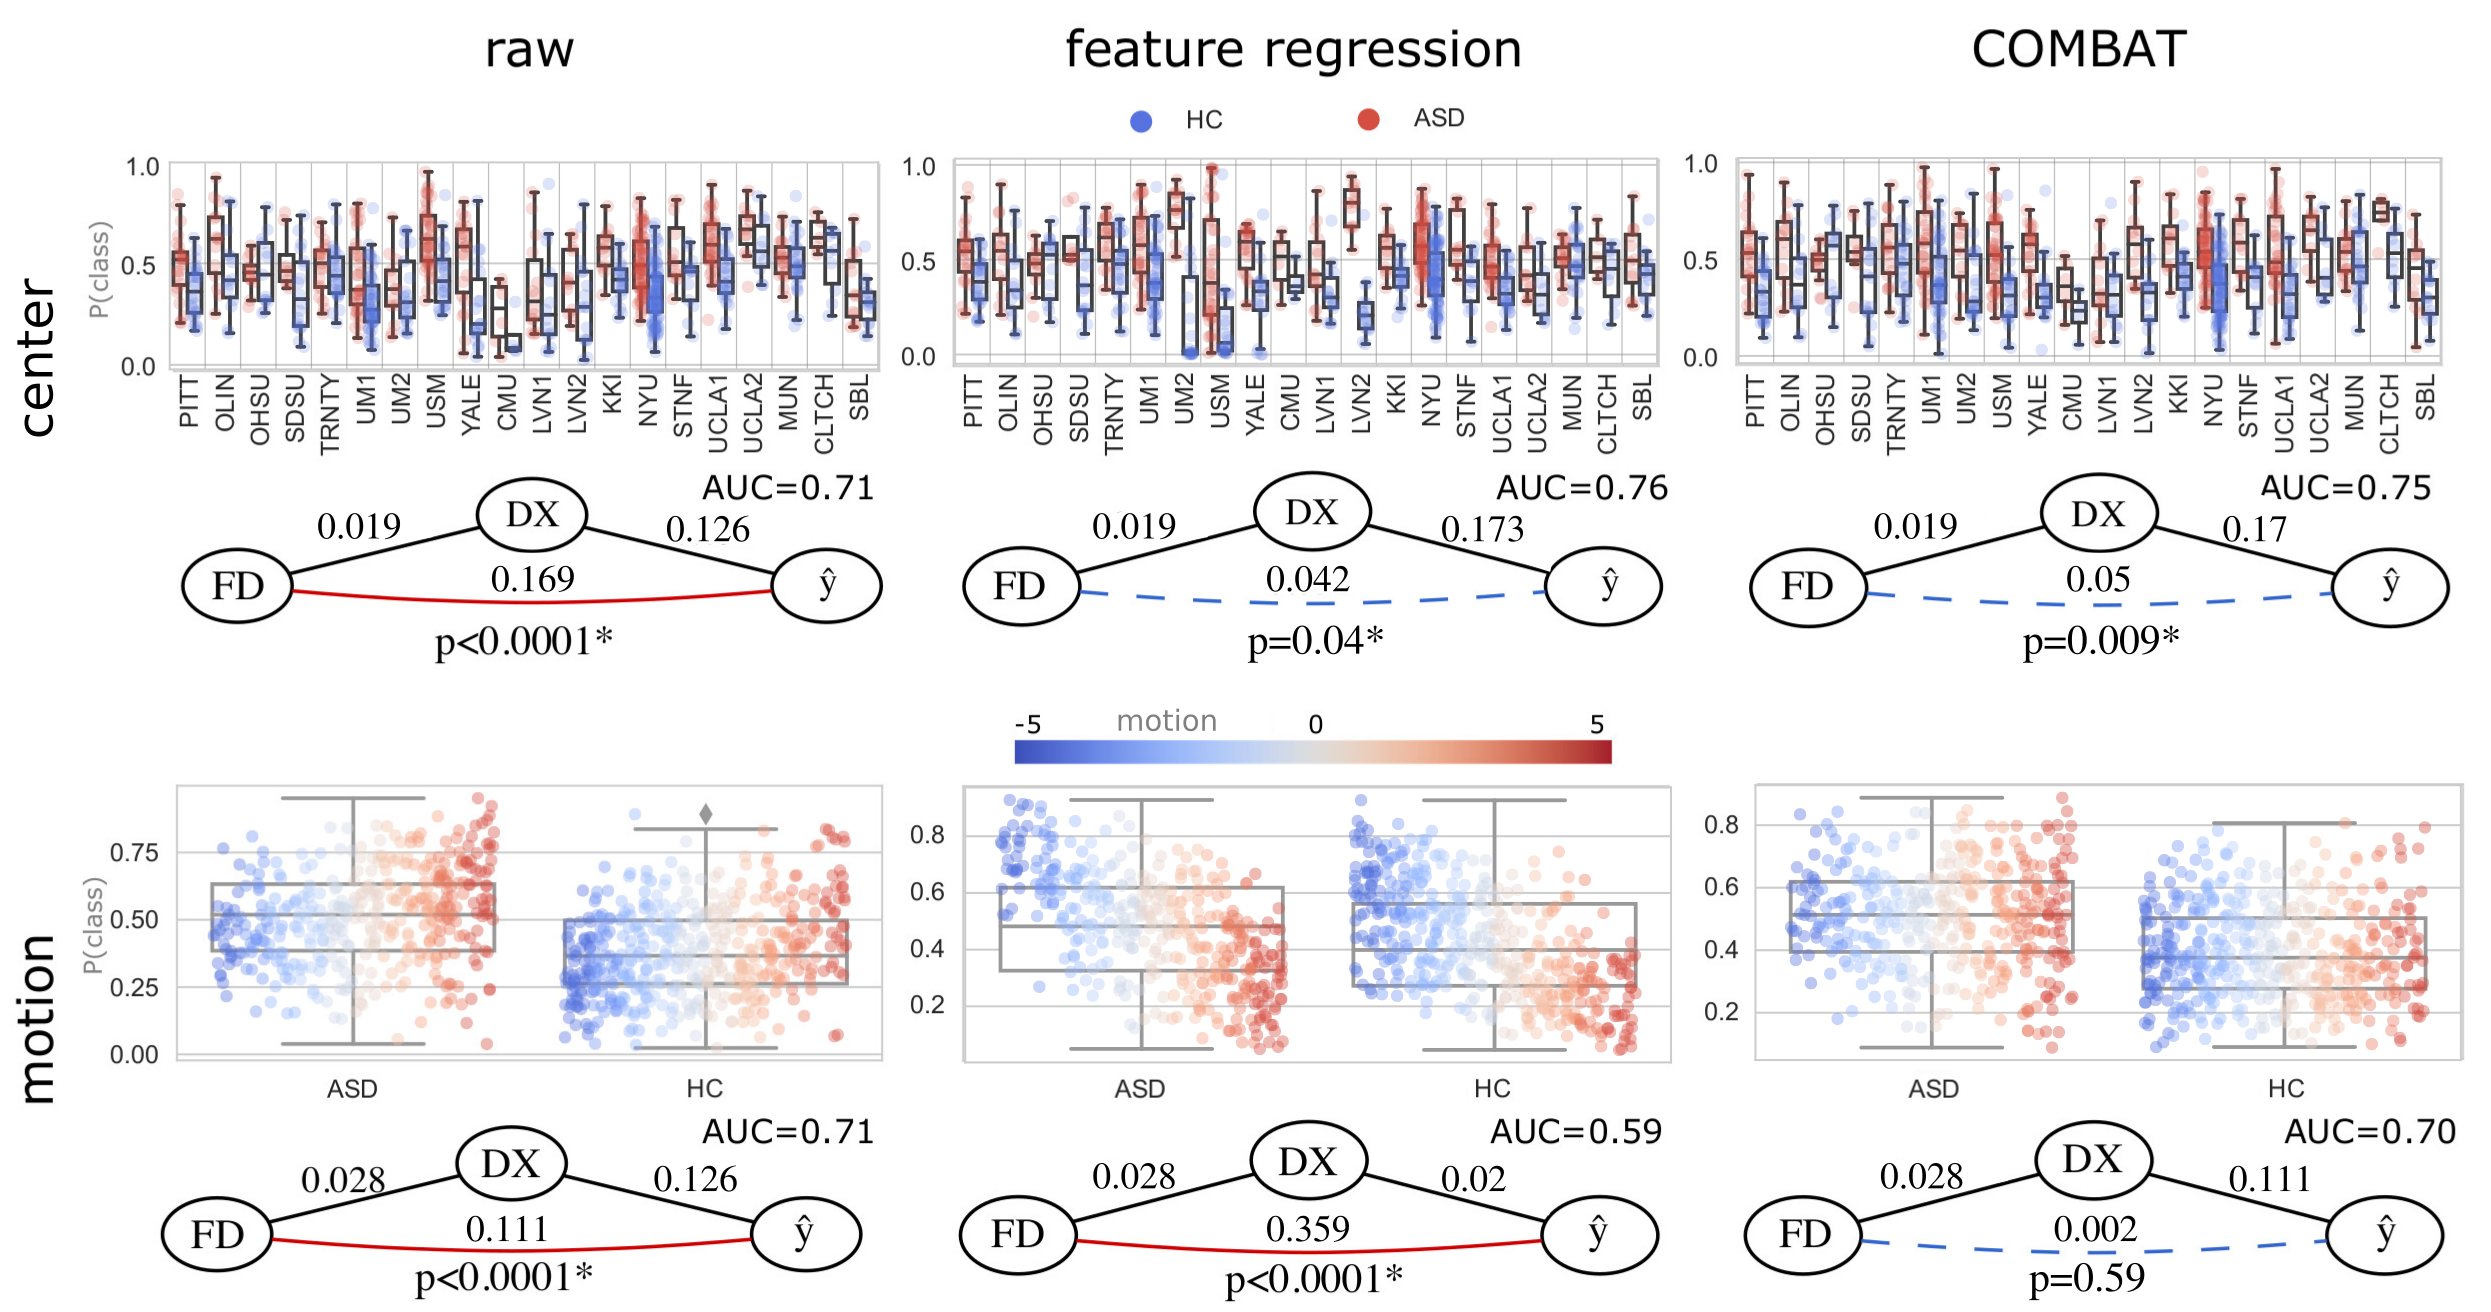
\includegraphics[width=0.75\paperwidth]{fig/fig_abide.png}
  \caption{\textbf{Center- and motion age-bias of ASD diagnosis prediction in the ABIDE dataset.} \\
  Boxplots and points show the predicted class probabilities (0: HC, 1: ASD), separately for the HC and ASD groups. In the top panel, predictions are plotted for each center separately and color indicates the true diagnosis (DX). AT the bottom plot, color indicates the normalized index of in-scanner motion (based on mean framewise displacement, mean FD). The proposed confounder test reveals significant center- and motion-bias in the model trained on the raw data (p<0.0001). While center bias seems to be effectively mitigated by feature regression, the same technique fails to remove motion-bias (actually introduces a paradoxical negative bias). COMBAT seems to effectively remove the effect of both confounders on the predictions and improves the predictive performance of the models in both cases.
  Relation between the observed ($\hat{y}$) and predicted IQ scores and the confounder variables is shown by the graphs as $R^2 values$. Solid red line between the confounder and the prediction means significant confounder bias, whereas blue dashed line denotes that confounder testing provided no evidence for bias. P-values are determined with the partial confound test. P-values of the full confound test were all less then 0.0001, i.e. confounder did not fully drive prediction for any of the models.
  }
  \label{fig:abide}
\end{figure}

Functional connectivity data from the ABIDE\citep{di2014autism} database was used to investigate the potential motion- and center-bias (as previously reported by e.g.\cite{spisak2014voxel, spisak2019optimal, gotts2013perils}) when training models that aim to predict ASD diagnosis.

Imaging center and in-scanner motion (normalized mean framewise displacement) were statistically significantly associated with ASD diagnosis ($R^2=0.019$ and $0.028$, respectively, $p<0.001$ for both, see also Table \ref{tab:unconditional-pvals}). The model trained on the raw (unadjusted) connectivity features predicted diagnosis with a medium effect size ($R^2=0.126$, $ROC AUC = 0.71$, $p<0.001$).
The partial confounder test revealed that the raw model was significantly biased both for age group and acquisition batch (both $p<0.0001$, see first column on Fig. \ref{fig:abide}). Several sites (e.g. Carnegine Mellon University, University of Leuven, Social Brain Lab UMC Groningen) and lower motion being weakly-moderately associated ($R^2=0.169$ and $0.111$, respectively) to a lower probability for the participant to be assigned to the ASD group by the model.

Both feature regression and COMBAT seemed to significantly attenuate the effect of imaging center, however the partial confound test still provided evidence for a significant center-bias ($p=0.04$ and $0.009$ for feature regression and COMBAT, respectively (second and third columns of the first row on Fig \ref{fig:abide}). 

When trying to mitigate the effect of in-scanner motion (bottom row on Fig \ref{fig:abide}), feature regression failed to remove the motion-bias from the model and, in fact, it introduced a paradoxical inverse dependence of the predictions on motion estimates. The partial confounder test successfully detected the resulting strong bias ($p<0.0001$). Applying COMBAT to remove the effect of motion (by using binned motion estimates), in turn, seemed to effectively mitigate motion-bias, as suggested by the partial confound test ($p=0.64$, bottom right panel of Fig \ref{fig:abide}).

Both feature regression and COMBAT considerably improved the predictive performance when mitigating center-effects ($R^2=0.111$ and $0.132$ and $AUC=0.76$ and $0.75$, respectively). With both feature regression and COMBAT, however, the effort of mitigating motion effects happened at the cost of a drop in predictive performance ($R^2=0.02$ and $0.111$ and $AUC=0.59$ and $0.70$, respectively)

The full confounder test was strongly significant ($p<0.0001$) for all models, except when regressing-out motion from the features ($p=0.09$), indicating that this model might have been (almost) exclusively driven by motion artifacts.

% tab:unconditional-pvals
\renewcommand{\arraystretch}{1.2}
\begin{table}
\centering
\begin{tabular}{lll|ll|ll|ll|ll} 
dataset & conf. & method & $R^2_{y, c}$ & $p_{y, c}$ & $R^2_{\hat{y}, c}$ & $p_{\hat{y}, c}$ & $R^2_{\hat{y}, y}$ & $p_{\hat{y}, y}$ & partial test & full test  \\
\hline
HCP & acq.  & raw      & 0.032 & <0.001 & 0.071 & <0.001  & 0.095 & <0.001 & \textbf{<0.0001} & <0.0001 \\
    &              & f.reg.    & & & 0.011 & 0.477 & 0.105  & <0.001  & 0.73 & <0.0001 \\
    &              & COMBAT    & & &0.013 & 0.4 & 0.122  & <0.001  & 0.65 & <0.0001\\
\hline
    & age   & raw       & 0.011 & 0.001  & 0.034 & <0.001  & 0.095  & <0.001 & \textbf{<0.0001} & <0.0001 \\
    &       & f.reg.    & & &0.004 & 0.052 & 0.114  & <0.001  & 0.2 & <0.0001 \\
    &       & COMBAT    & & &0.005 & 0.048 & 0.121 & <0.001 & 0.16 & <0.0001 \\
\hline
ABIDE   & center   & raw       & 0.019  & <0.001 &  0.169 & <0.001& 0.126     & <0.001 & \textbf{<0.0001} & <0.0001 \\
        &          & f.reg.    &  & &  0.042 & 0.007 & 0.173     & <0.001 & \textbf{0.04} & <0.0001 \\
        &          & COMBAT    &  & &  0.05 & 0.001 & 0.17     & <0.001 & \textbf{0.009} & <0.0001 \\
\hline
        & motion   & raw       & 0.028 & <0.001 & 0.111    &  <0.001 & 0.126    & <0.001 & \textbf{<0.0001} & <0.0001 \\
        &          & f.reg.    & & & 0.359    & <0.001  & 0.02   & <0.001 & \textbf{<0.0001} & 0.1 \\
        &          & COMBAT    & & &  0.002 & 0.19 & 0.111     & <0.001 & 0.59 & <0.0001 \\
    

\end{tabular}
\caption{\label{tab:unconditional-pvals} Unconditioned coefficients-of-determination, the corresponding p-values and the p-values of the partial and full confounder tests for all investigated confounder-mitigation methods. Significant confoudner bias is denoted by bold font.}
\end{table}

%%%%%%%%%%%%%%%%%%%%%%%%%%%%%%%%%%%%%%%%%%%%%%%%%%%%%%%%%%%%%%%%%%%%%%%%%%%
\section{Discussion}

The assessment of confoudner bias via conditional independence testing is a very appealing solution due to its simplicity and applicability in a wide variety of settings. However, statistical testing of conditional independence is challenging: analogs of bivariate (unconditioned) non-parametric tests can give invalid results even by slight violations of normality and linearity\citep{korn1984ranges} (see an example on Fig. \ref{fig:sim-h0-demo}). While the magnitude of this problem may not be fully appreciated in case of predictive model diagnostics, the "no free lunch theorem" (i.e. the nonexistence of a uniformly valid conditional independence test)\cite{shah2020hardness} clearly implies that conditional independence-based confoudner bias testing must be designed so that its suitability for the particular problem may be judged easily.

In this paper, I have proposed a solution for confounder testing, which was designed to be suitable for the specific characteristics of the 'confoudner problem' in predictive modelling. Namely, the proposed approach places assumptions only about the conditional distribution of the confoudner and the target variables, as required by the applied generalized additive\cite{hastie1987generalized} or multinomial logistic model\cite{bennett1966multiple, jones1975proability}. In biomedical research practice, these are variables that are often subject to descriptive (and often parametric) statistical analysis, as well. Accordingly, usually there is sufficient expert knowledge about the applicability of the required assumptions and data acquisition is probably already designed so that the assumptions are likely fulfilled.
Of key importance, the proposed solution is \emph{absolutely assumption-free} regarding the distribution and dependency of the prediction output, which is, in most of the cases, unknown and can often be expected to be non-normal and/or non-linear (due to e.g model regularization)\citep{garcia2009study, kristensen2017whole}. 
This property distinguishes the approach from other alternatives as it guarantees a valid type-I error control even in cases of non-normally and non-linearly dependent predictions, i.e. in cases where Pearson and Spearman partial correlations, and many other methods fail.

The proposed approach gives rise to two different statistical tests for testing confoudner bias: the \emph{full confounder test} probes whether the model's predictive performance can be attributed exclusively to the confounder and the \emph{partial confounder test} investigates whether the model utilizes any confounder-variance in the predictions, when controlled for the target variable. 
The tests can be applied for arbitrary classification or regression models, without having to re-fit the model, that is, with a negligible extra computational cost.

As expected from theory, both tests displayed a valid type I error control and a high, practically relevant statistical power in the simulations, even if both the predictions and the confounder are non-normally and/or non-linearly dependent on the target variable (except extreme non-normality), confirming the tests' can be deployed in most predictive modelling scenarios. While different biomedical applications might consider different amounts of bias to be relevant, the presented results can serve as a basis for power calculation in order to identify the necessary sample size for proper model diagnostics.
Validity, power and robustness renders the proposed tests as unprecedented tools for model diagnostics in a wide spectrum of predictive modelling scenarios.

%In biomedical research, confounder-bias has previously often been investigated (if investigated at all) simply by testing the (unconditioned) association between the confounder variable and the predictive values, see e.g.\citep{spisak2020pain}. However, the significance of the unconditioned association does not necessarily imply a significant confound-bias of the model, especially if the confounder is also associated to the true target variable. In this case, namely, the model still might not be directly driven by the confounder and the dependence of the predictions on the confounder might be only marginal, to be explained solely by the confounder-target association. 
%Two examples for this situation can be found in the presented analysis of real data; when applying COMBAT to mitigate age-bias in the HCP data and when regressing out the center-effect from the ABIDE data (see Table \ref{tab:unconditional-pvals}).
%These examples clearly indicate that guiding model diagnostics based on unconditioned associations between the confounder and the model output might result in overly strict decisions. More realistic is to aim at models that allow a reasonable degree of marginal confounder-association of the predictions, but are likely not directly driven by confounder-information, i.e. the prediction-confounder association is proportional to, and can be fully explained by, the target-confounder association.
%Put simply, this is what is tested by the proposed partial confounder test.

%Obviously, a true confounder bias might still be present in the model, even if the the target-confounder association likely explains the prediction-confounder association, i.e. the model might still use the confounder's effect on the features (e.g artifacts) to construct the corresponding part of the variance in the prediction. Nevertheless, in most of the cases, it does not seem likely that the model, at the same time, (i) misses that specific "part" of the target variable's variance in the features that is shared with the confounder (ii) captures exclusively that component of the confounder's variance in the features that is needed to mimic an unbiased model.
%Usually a much more plausible explanation is that a direct confounder effect in the model output is simply negligible (e.g because it is not to be found in the features after confound mitigation).

A characteristic example for the potential areas of applications is the novel field of "predictive neuroscience", where applying predictive modelling and machine learning on functional neuroimaging data holds great potential for both revolutionizing our understanding of the physical basis of mind and delivering clinically useful tools for diagnostics or therapeutic decision making\citep{woo2017building, wager2013fmri, spisak2020pain}. However, the presence of confounders typical for biomedical research (e.g. sample demographics, center-effects) and specific to the data acquisition and processing approach (e.g. imaging artifacts) presents a great challenge to these efforts.
The usefulness of the proposed tests is demonstrated in two such examples, using the HCP\citep{van2013wu}  and the ABIDE\citep{di2014autism} datasets.
%First, functional connectivity data from the Human Connectome Project (HCP)\citep{van2013wu} was used to build predictive models of fluid intelligence and to test for the previously discussed confounding effect of age\citep{lohmann2021predicting, dubois2018distributed} and,  additionally, the - somewhat underdiscussed - batch-like effect of acquisition date of the data within the course of the data acquisition process.
%Second, functional connectivity data from the ABIDE\citep{di2014autism} database was used to investigate the potential motion- and center-bias (as previously reported by e.g.\cite{spisak2014voxel, spisak2019optimal, gotts2013perils}) when training models that aim to predict ASD diagnosis.
%The hypothesised confounder effects were clearly present in both datasets.

In case of the HCP dataset, the weak but statistically significant confounder effect of age on fluid intelligence is in line with previous findings\citep{dubois2018distributed, lohmann2021predicting}) could likely exaggerate to a serious bias when testing the model on data of participants outside of the - relatively narrow - age range of the HCP sample. In this case, the bias would likely significantly harm the out-of-sample generalizability of this model. The bias of the same model to 'acquisition batch' (phase of the study the acquisition belongs to) can also be problematic and it has not yet been thoroughly discussed in case of the HCP dataset. There can be manifold reasons for the observed bias. Fluid intelligence of the included participants might be, for instance, affected by a changing selection bias during participant recruitment (e.g. as a consequence of the human connectome project receiving an increasing degree of public interest during its course, the sociodemographic and educational characteristics of the volunteer sample might have changed over time). To explain the associated change in the target variable, the model might utilise changing characteristics of the imaging data (caused by e.g. slight changes in the calibration settings of the measuring equipment or the changing level of experience of the research staff). This is obviously undesirable for any brain-based predictive model of fluid intelligence.

In the ABIDE dataset, neither the medium-strong center-bias nor the age-bias is surprising but both are obviously problematic for a diagnostic model of ASD. For instance the model trained on the raw (unadjusted) features - depending on the calibration of the predicted class probabilities - might classify all participants form e.g. the CMU (Carnegie Mellon University) center as neurotypical control participants. Similarly, the models biased by motion - next to having questionable neuroscientific validity - might systematically fail in populations with a tendency for higher in-scanner motion, e.g. due to atypical motor function (as known e.g. for ADHD\citep{eloyan2012automated}).
 
 The partial confounder test provided quantitative, statistically rigorous metrics for assessing the effectiveness of the investigated confounder mitigation techniques. In the HCP data, it revealed that both the acquisition bias and the age bias was very effectively removed by both feature regression and COMBAT (p>0.05 for all). Given the high power of the test at the sample sizes of the HCP dataset ($N=999$), any remaining confounder-bias is most probably very safely negligible and well out of the range of practical relevance.
 
On the other hand, the partial confoudner test also showed, that the performance of the investigated confound mitigation techniques is much less convincing for the ABIDE dataset. The center bias of the classification in this massively multi-center dataset was, namely, found to be significant, even after feature regression and COMBAT. Nevertheless, the p-values returned by the partial confounder test increased, in both cases, with two orders of magnitude as compared to the case with raw features, suggesting that a large part of center effects was still successfully removed by both approaches. Although determining the relevance of the remaining bias is out of the scope of this paper, significant p-values of the partial confounder test generally suggest that these models require more effective data harmonization.

Motion-bias in the ABIDE dataset was not detectable anymore after COMBAT, but remained highly significant after feature regression.
Interestingly, in the latter case, the association between the confounder and the predictions become even stronger than before but with an opposite sign. Meanwhile, the prediction performance substantially dropped (although still remained statistically significant). 
A possible explanation to these phenomena is that in-scanner motion, as previously described\citep{fournier2010motor, anzulewicz2016toward}, has manifold links to ASD and, therefore, regressing out motion estimates from the connectivity features might eliminate a significant amount of signal-of-interest (especially in functional connections that are themselves directly associated with motor deficits in ASD).
This effect might be boosted by the previously reported "residual motion artifacts" and their regional interactions\citep{spisak2014voxel} and raises caution for using feature regression to mitigate the effect of motion artifacts and similarly complex confounders.
 As COMBAT was originally developed for harmonizing effects of categorical variables (e.g. center or batch), its application for continuous confounder variables is not trivial. The presented method of inputting the binned "motion groups" into COMBAT resulted in an efficient removal of motion-bias and, at the same time, preserved a significant amount of signal-of-interest. 
 Nevertheless, inputting discretized versions of continuous variables into COMBAT might be sub-optimal and raises further questions e.g regarding the optimal number of bins used during the discretization.
 
 In sum, the application of the \emph{partial} confounder test on the real data examples suggests that confounder-bias should be much more carefully investigated and reported in studies utilizing predictive modelling and machine learning as (i) variables as trivial as the date of the acquisition can cause significant model-bias and (ii) in certain situations, a sufficient mitigation of confounder-bias requires more effective solutions than feature regression and COMBAT and (iii) in some cases confoudner mitigation can - paradoxically - introduce more bias. The partial confounder test can be considered as a useful, objective benchmark to guide the search for a suitable confounder mitigation approach for every dataset.
 Regarding the \emph{full} confounder test; while the real data examples in this paper were not typical cases of its potential applications, it has still provided important insights into model biases. Namely, in the case of the aforementioned paradox motion-regression model in the ABIDE dataset, the full confounder test did not provide any evidence that the model captures any extra variance over that explained by the confounder ($p=0.1$). In other words, the test accepted the null hypothesis of full model bias, suggesting that this model might be, in fact, almost exclusively driven by motion artifacts.
This example highlights that the full confounder test might become useful in exploratory phases of model development, where models might be still severely biased by various confounders and the questions is whether there is any biomedically relevant signal captured by the model, at all.


%%%%%%%%%%%%%%%%%%%%%%%%%%%%%%%%%%%%%%%%%%%%%%%%%%%%%%%%%%%%%%%%%%%%%%%%%%%
\section{Conclusion}

The lack of rigorous statistical tests for confounder-bias significantly hampers the development of predictive models in many fields of research. Although several approaches for mitigating the effects of counfounder variables in machine learning have been recently proposed, these can potentially remove signal-of-interest together with the confounder signal and an informed decision about confound mitigation strategy is impossible without a proper test of confounder-bias.

To fill this critical gap in predictive model development, here I proposed two novel tests, the \emph{partial} and the \emph{full confounder tests}, which probe the null hypotheses of 'no confounder-bias' and 'full confounder-bias', respectively. Both approaches are based on a recently published framework for conditional permutation testing, with a mathematical justification of valid type I error control and with assumptions that are easy to meet in most predictive modelling scenarios. The tests have a minimal computational overhead; as re-fitting the model is not required.

As demonstrated on functional brain connectivity-based predictive models of fluid intelligence and autism, the tests can guide the optimization of the confound mitigation strategy and allow quantitative, statistical assessment of the robustness, generalizability and neurobiological validity of predictive models in biomedical research.
Given their simplicity, wide applicability, high statistical power and computationally effective implementation (available in the  python package \emph{mlconfound}\footnote{\href{https://mlconfound.readthedocs.io}{https://mlconfound.readthedocs.io}}), the partial and full confoudner tests can become widespread tools that pave the way for the development of clinically useful machine learning biomarkers.

\newpage
%%%%%%%%%%%%%%%%%%%%%%%%%%%%%%%%%%%%%%%%%%%%%%%%%%%%%%%%%%%%%%%%%%%%%%%%%%%
%TC:ignore
\section{Methods}
\label{sec:methods}

\subsection{Notation and Background}

In a predictive modelling setting, let $\y$ denote the target variable, $\yhat$ denote model output, i.e. the predictions for $\y$ and let $\c$ denote a variable which is considered as a confounder (see Fig. \ref{fig:schematic}B). Let us assume, furthermore, that $\y$, $\yhat$ and $\c$ consist of independent and identically distributed (IID) data points $(y_i, \hat{y}_i, c_i) \in Y \times \hat{Y} \times C$ for $i=1, \dots , n$ so that $\y=(y_1, \dots ,y_n)$, $\yhat=(\hat{y}_1, \dots, \hat{y}_n)$ and $\c=(c_1, \dots, c_n)$. 

Depending on the research question, the direct influence of $\c$ on the model predictions $\yhat$ is subject to be kept at a negligible level or it is to be proven that, at least, the model is not completely driven by $\c$.

Obviously, a strong association between $\yhat$ and $\c$ might indicate that the model is biased; its predictions are driven by the confounder rather than information about the target variable.
Testing unconditional independence ($\yhat \independent \c$) between $\yhat$ and $\c$ (or any of the $\y$, $\yhat$, $\c$ variables) is, however, insufficient for the proper characterization of confounder-bias in predictive modelling.
For instance, even if $\yhat \independent \c$ is false, $\yhat$ might be only marginally dependent on $\c$, due to the dependence of both on $\y$. In other words, if the target variable $\y$ displays a true association to the confounder variable $\c$, a model that is completely blind to $\c$ (i.e not confounded at all) might still provide outputs $\yhat$ that are significantly associated with $\c$.

\subsubsection*{Conditional independence for testing confounder bias}

Instead of focusing on the unconditional independence between the confounder and the predictions, we shall consider the \emph{conditional independence} between $\yhat$ and $\c$ given $\y$ (written as $\yhat \independent \c | \y$) which, by definition \citep{dawid1979conditional}, means that $\mathbb{P}(\yhat, \c|\y) = \mathbb{P}(\yhat|\y)\mathbb{P}(\c|\y)$. The statistical test with this null hypothesis will be referred to as the \emph{partial confounder test}.

Alternatively, one might also be interested in testing $\yhat \independent \y | \c$. We will refer to the corresponding test as the \emph{full confounder test}.

 Conditional independence - in its general form - lies at the heart of several fundamental concepts in statistics and  plays an increasingly important role in various fields of applied statistics, particularly in biomedical applications\citep{spirtes2000causation, fiedler2011mediation, peters2016causal, candes2016panning}. Recently,\cite{shah2020hardness} have raised important concerns regarding conditional independence testing.
 Their "no free lunch" theorem implies that, without placing some assumptions on the joint distribution of $(\y, \yhat, \c)$, conditional independence testing is effectively impossible. In other words, neither the full nor the partial confounder tests can be constructed so that - for all distributions - they provide a valid type I error control and, at the same time, a non-trivial statistical power.

This result stands in strong contrast to \emph{unconditional} independence testing - where permutation tests \citep{pitman1937significance, fisher1942189}, provide a general, distribution-free solution - and it has important implications for confounder testing in predictive modelling where the distribution of the model outputs (conditioned on the target variable) - depending on the applied machine learning model - is unknown and often non-normal and non-linear.

One of the trivial candidates for the task, partial correlation, for instance assumes that all involved variables are multivariate Gaussian and - as to be shown below - even its Spearman-based variant is unable to tolerate relatively small deviations from normality and linearity.

Recently,\cite{candes2016panning} and\cite{berrett2020conditional} have demonstrated that valid and powerful conditional independence tests can be constructed with inputting distributional information about only two (out of the three) variables.
Specifically, the conditional permutation test (CPT) of Berrett and colleagues samples from a non-uniform distribution over the set of possible permutations $\pi$ of one of the variables, based on its conditional distribution of the other variable. Thereby, it incorporates the information available on the conditional distribution of interest into the permutation-based inference in a statistically valid manner. Moreover, as shown in this paper, CPT can be combined with a generalized additive model (GAM) to handle non-linear relationships, rendering it as an appealing candidate for testing confounder effects in predictive modelling.

As many related papers, the work of\cite{berrett2020conditional} was formalized as a (semi-)supervised learning approach, where $X$ is a set of predictors (features), $Y$ is the target variable and $Z$ is a potential confounder. In this setting, testing the null hypothesis $X \independent Y | Z$ aims to determine, whether the features $X$ still affect $Y$, when controlling for $Z$.
For instance, in genome-wide association studies, CPT can be used to determine whether a particular genetic variant $X$ affects a response $Y$ such as disease status or some other phenotype, even after controlling for the rest of the genome, encoded in $Z$.

In this paper, a different setting is considered, where the supervised learning model is already fitted and we are focusing on model diagnostics, by testing the triplet $(\y,\yhat, \c)$. 
The conceptual difference between the original and the proposed application of CPT is depicted on Fig. \ref{fig:schematic}.

% fig:schematic
\begin{figure}
  \centering
  \resizebox{0.75\columnwidth}{!}{%
\tikzset{every picture/.style={line width=0.75pt}} %set default line width to 0.75pt        


\tikzset{every picture/.style={line width=0.75pt}} %set default line width to 0.75pt        

\begin{tikzpicture}[x=0.75pt,y=0.75pt,yscale=-1,xscale=1]
%uncomment if require: \path (0,300); %set diagram left start at 0, and has height of 300

%Shape: Circle [id:dp12907748114570317] 
\draw   (299.5,107) .. controls (299.5,93.19) and (310.69,82) .. (324.5,82) .. controls (338.31,82) and (349.5,93.19) .. (349.5,107) .. controls (349.5,120.81) and (338.31,132) .. (324.5,132) .. controls (310.69,132) and (299.5,120.81) .. (299.5,107) -- cycle ;
%Shape: Circle [id:dp12318976880062338] 
\draw   (397,39) .. controls (397,25.19) and (408.19,14) .. (422,14) .. controls (435.81,14) and (447,25.19) .. (447,39) .. controls (447,52.81) and (435.81,64) .. (422,64) .. controls (408.19,64) and (397,52.81) .. (397,39) -- cycle ;
%Shape: Circle [id:dp2655574667622329] 
\draw   (202,39) .. controls (202,25.19) and (213.19,14) .. (227,14) .. controls (240.81,14) and (252,25.19) .. (252,39) .. controls (252,52.81) and (240.81,64) .. (227,64) .. controls (213.19,64) and (202,52.81) .. (202,39) -- cycle ;
%Curve Lines [id:da9340239406716428] 
\draw    (250,28) .. controls (292,20) and (364,22) .. (400,28) ;
%Curve Lines [id:da6958426380393512] 
\draw    (239,61) .. controls (249,76) and (276,99) .. (299.5,107) ;
%Curve Lines [id:da8565840155201192] 
\draw    (349.5,107) .. controls (365,101) and (403,71) .. (410,60) ;

%Shape: Circle [id:dp9753164043561875] 
\draw   (475.5,257) .. controls (475.5,243.19) and (486.69,232) .. (500.5,232) .. controls (514.31,232) and (525.5,243.19) .. (525.5,257) .. controls (525.5,270.81) and (514.31,282) .. (500.5,282) .. controls (486.69,282) and (475.5,270.81) .. (475.5,257) -- cycle ;
%Shape: Circle [id:dp6395662810469516] 
\draw   (573,189) .. controls (573,175.19) and (584.19,164) .. (598,164) .. controls (611.81,164) and (623,175.19) .. (623,189) .. controls (623,202.81) and (611.81,214) .. (598,214) .. controls (584.19,214) and (573,202.81) .. (573,189) -- cycle ;
%Shape: Circle [id:dp786541411329625] 
\draw   (378,189) .. controls (378,175.19) and (389.19,164) .. (403,164) .. controls (416.81,164) and (428,175.19) .. (428,189) .. controls (428,202.81) and (416.81,214) .. (403,214) .. controls (389.19,214) and (378,202.81) .. (378,189) -- cycle ;
%Curve Lines [id:da22693900064180195] 
\draw    (426,178) .. controls (468,170) and (540,172) .. (576,178) ;
%Curve Lines [id:da6720989194231959] 
\draw    (415,211) .. controls (425,226) and (452,249) .. (475.5,257) ;
%Curve Lines [id:da8140666812849395] 
\draw    (525.5,257) .. controls (541,251) and (579,221) .. (586,210) ;
%Shape: Circle [id:dp471386481785639] 
\draw   (50,256) .. controls (50,242.19) and (61.19,231) .. (75,231) .. controls (88.81,231) and (100,242.19) .. (100,256) .. controls (100,269.81) and (88.81,281) .. (75,281) .. controls (61.19,281) and (50,269.81) .. (50,256) -- cycle ;
%Shape: Rectangle [id:dp8617145222488287] 
\draw   (156,237) -- (240,237) -- (240,277) -- (156,277) -- cycle ;
%Shape: Circle [id:dp8776576784951928] 
\draw   (290,256) .. controls (290,242.19) and (301.19,231) .. (315,231) .. controls (328.81,231) and (340,242.19) .. (340,256) .. controls (340,269.81) and (328.81,281) .. (315,281) .. controls (301.19,281) and (290,269.81) .. (290,256) -- cycle ;
%Shape: Circle [id:dp2868603849402189] 
\draw   (174,190) .. controls (174,176.19) and (185.19,165) .. (199,165) .. controls (212.81,165) and (224,176.19) .. (224,190) .. controls (224,203.81) and (212.81,215) .. (199,215) .. controls (185.19,215) and (174,203.81) .. (174,190) -- cycle ;
%Callout Right Arrow [id:dp26184503306970397] 
\draw   (46.55,225.27) -- (106,225.27) -- (106,250) -- (133,250) -- (133,241) -- (155.55,255.27) -- (133,269.55) -- (133,260.55) -- (106,260.55) -- (106,285.27) -- (46.55,285.27) -- cycle ;
%Right Arrow [id:dp7986276189609152] 
\draw   (240,250) -- (268,250) -- (268,241) -- (290,255.5) -- (268,270) -- (268,261) -- (240,261) -- cycle ;
%Shape: Circle [id:dp9535423837564185] 
\draw   (50,190) .. controls (50,176.19) and (61.19,165) .. (75,165) .. controls (88.81,165) and (100,176.19) .. (100,190) .. controls (100,203.81) and (88.81,215) .. (75,215) .. controls (61.19,215) and (50,203.81) .. (50,190) -- cycle ;
%Straight Lines [id:da6172567079022628] 
\draw    (75,215) -- (75,231) ;
%Straight Lines [id:da8731068989736062] 
\draw    (198,238) -- (198,215) ;

% Text Node
\draw (165,251) node [anchor=north west][inner sep=0.75pt]   [align=left] {ML model};
% Text Node
\draw (9,6) node [anchor=north west][inner sep=0.75pt]   [align=left] {\textbf{A}};
% Text Node
\draw (9,146) node [anchor=north west][inner sep=0.75pt]   [align=left] {\textbf{B}};
% Text Node
\draw (494,252.4) node [anchor=north west][inner sep=0.75pt]    {$\c$};
% Text Node
\draw (591.5,180.4) node [anchor=north west][inner sep=0.75pt]    {$\yhat$};
% Text Node
\draw (396,184.4) node [anchor=north west][inner sep=0.75pt]    {$\y$};
% Text Node
\draw (484,198) node [anchor=north west][inner sep=0.75pt]   [align=left] {CPT};
% Text Node
\draw (67,251.4) node [anchor=north west][inner sep=0.75pt]    {$X$};
% Text Node
\draw (308.5,247.4) node [anchor=north west][inner sep=0.75pt]    {$\yhat$};
% Text Node
\draw (191,185.4) node [anchor=north west][inner sep=0.75pt]    {$\y$};
% Text Node
\draw (318,102.4) node [anchor=north west][inner sep=0.75pt]    {$Z$};
% Text Node
\draw (415.5,34.4) node [anchor=north west][inner sep=0.75pt]    {$Y$};
% Text Node
\draw (219,34.4) node [anchor=north west][inner sep=0.75pt]    {$X$};
% Text Node
\draw (308,48) node [anchor=north west][inner sep=0.75pt]   [align=left] {CPT};
% Text Node
\draw (68,185.4) node [anchor=north west][inner sep=0.75pt]    {$\c$};


\end{tikzpicture}

    }
  \caption{Schematic diagram of using CPT in a predictive modelling context. \\ \textbf{(A)} CPT was originally proposed to be used on the feature variable $X$, target variable $Y$ and confounders $Z$. \textbf{(B)} The proposed use of CPT in predictive modelling requires the model to be fitted first, to obtain the model's prediction $\yhat$ on $\y$. CPT is then utilized on the triplet $(\y, \yhat, \c)$, to test hypotheses $\yhat \independent \c | \y$ or $\y \independent \yhat | \c$.}
  \label{fig:schematic}
\end{figure}

Within this setting, conditional independence testing and, specifically, the framework of conditional permutation testing allows investigating three different null hypotheses corresponding to the $(\y, \yhat, \c)$ triplet. As listed in Table \ref{tab:conditional-independence-cases}, testing the null hypothesis $\y \independent \yhat | \c$ (option 1, full confounder testing) investigates whether the model predictions are likely explainable solely with the confounder, i.e. whether the model is exclusively confounder-driven. Testing $\y \independent \c | \yhat$ (option 2) addresses the question whether the model captures all the variance in $c$ when predicting $y$. Testing the null hypothesis $\yhat \independent \c | \y$ (option 3, partial confounder testing) examines, whether the dependence of the model output on the confounder can likely be explained by the confounder's dependence on the target variable, i.e. whether there is any confounder bias in the model.

% tab:conditional-independence-cases
\renewcommand{\arraystretch}{1.2}
\begin{table}[]
\centering
\begin{tabular}{l|rp{60mm}|c|>{\centering\arraybackslash}m{30mm}}
 &  & H0  & assumption needed for: & no assumptions about the distribution of: \\
\hline
\textbf{1.} & $\yhat \independent \y | \c$ \quad  & full confounder test: model exclusively driven by the confounder & $Q(\y|\c)$ & $(\yhat,\y), (\yhat, \c)$ \\
%\hline
\textbf{2.} & $\y \independent \c | \yhat$ \quad & model captures all variance in the confounder (not of interest) & $Q(\c|\yhat)$ & $(\y, \c), (\y, \yhat)$ \\
%\hline
\textbf{3.} & $\yhat \independent \c | \y$  \quad &  partial confounder  test: model not directly driven by the confoudner & $Q(\c|\y)$ & $(\yhat, \c), (\yhat, \y)$ \\
\end{tabular}
\caption{\label{tab:conditional-independence-cases} Possibilities when testing conditional independence in potentially biased predictive models. \\The table lists the three possible null hypotheses (H0), and the variables where assumption about the joint/conditional distributions is required/not required.   ($\y$: prediction target, $\yhat$: predictions, $\c$: confounder variable) }
\end{table}

Option 3, i.e. partial confounder testing is typically of interest when testing confounder bias of predictive models. Option 1, i.e. full confounder testing, might be also useful in diagnostics of predictive models, especially in the exploratory phase of model construction. Option 2 seems less appealing for model diagnostics and importantly, in this case the proposed variety of the CPT framework does not allow constructing a test which is non-parametric on $\yhat$.

In the following section, CPT is adapted for partial confounder testing (option 3). For an overview, see Fig. \ref{fig:overview}. The formulation of the full confounder test (option 1) is analogous and given in Supplementary Material \ref{sup:full-test}.
\subsubsection*{The partial confounder test}

The partial confounder test generates a null-distribution for an arbitrary predefined test statistic $T(\y,\yhat,\c)$ by sampling permutation based 'copy' of $\c$,

\begin{equation}
    c_i^{(j)} \sim Q(\cdot|y_i)
     \label{eq:cond-copy}
\end{equation}

where, $Q(.|y)$ denotes the conditional distribution of $\c$ given $\y=y_i$ and $j=1,\dots, m$ indexes the 'copy' of $\c$ so that

$$ \c^{(j)} = (c_1^{(j)}, \dots, c_n^{(j)}) = (c_{\pi_1^{(j)}}, \dots, c_{\pi_n^{(j)}}) =  \c_{\boldsymbol{\pi}^{(j)}} $$

is a permutation of the original vector $\c = (c_1, \dots, c_n)$, with its elements reordered according to the permutation $ \boldsymbol{\pi} \in S_n$ where $S_n$ denote the set of all permutations on the indices $\{1,\dots,n\}$.

As shown in\citep{berrett2020conditional}, to ensure that Eq. \ref{eq:cond-copy} holds, the $\c_{\boldsymbol{\pi}^{(j)}}$ copies must be drawn so that:

\begin{equation}
    \label{eq-pperm}
    \mathbb{P}(\boldsymbol{ \pi }^{(j)} = \boldsymbol{ \pi } | \y,\yhat,\c) = \frac{q^n(\c_{\boldsymbol{ \pi }} | \y)}{\sum_{\boldsymbol{ \pi } ' \in S_n} q^n(\c_{\boldsymbol{ \pi } ' } | \y)}
\end{equation}


that is, according to the $q^n(\cdot|\y) := q(\cdot | y_1) \dots q(\cdot|y_n)$ product density corresponding to the conditional distribution $Q(\cdot|\y)$. Note that Eq. \ref{eq-pperm} does not necessarily assume a continuous distribution.

This mechanism creates copies $\c^{(1)}, \dots ,\c^{(m)}$ so that under the null hypothesis ($\yhat \independent \c | \y$), the triples 

$$(\y,\yhat,\c), (\y, \yhat, \c^{(1)}),\dots, (\y, \yhat, \c^{(m)})$$

are all identically distributed and so are the 

$$T(\y,\yhat,\c), T(\y, \yhat, \c^{(1)}),\dots,T(\y, \yhat, \c^{(m)})$$

test statistics, as well.

As long as the numerator of Eq. \ref{eq-pperm} is non-zero for all $c_\pi \in C$ and $y \in Y$, the conditional permutations constitute an algebraic group, thus, as shown by\citep{hemerik2018exact}, an unbiased estimate of the p-value under the null can be obtained as:
$$ p= \frac{\sum_{j=1}^m \mathbb{1} \{T(\y, \yhat, \c^{(j)}) \geq T(\y, \yhat, \c) \}  }{m}$$

While the group property of the conditioned permutations provides a straightforward proof for the validity of the approach, for an alternative verification see the proof of Theorem 1 in\citep{berrett2020conditional}.

The required permutations could be theoretically sampled with a simple Metropolis-Hastings algorithm that draws uniformly from $S_n$ at random. However, this way the acceptance ratio would be extremely low, even for moderate $n$ (except there is very low dependence of $\c$ on $\y$), resulting in slow mixing times. The partial confounder test can be, however, efficiently implemented with the parallelized pairwise Markov-Chain Monte Carlo sampler of\cite{berrett2020conditional} (Algorithm 1), that draws disjoint pairs in parallel and decides whether or not to swap them randomly, according to the odds ratio calculated from the conditional densities belonging to the original and swapped data. The acceptance odds ratio of swapping indices $i$ and $j$ is:

\begin{equation}
\frac{ q(c_j | y_i) q(c_i | y_j)}{q(c_i | y_i) q(c_j | y_j) }
=
\ell(c_j | y_i) + \ell(c_i | y_j) - \ell(c_i | y_i) - \ell(c_j | y_j) 
\label{eq:accept-odds}
\end{equation}

where $\ell$ denotes the log-likelihood.

In their Theorem 2,\cite{berrett2020conditional} verify that the resulting Markov Chain yields the desired stationary distribution, even if the number of steps is small.

\subsubsection*{Conditional log-likelihood}


Obtaining a relatively accurate, independent estimate of $D(\cdot|\y)$ (of any shape) for CPT inference is important. Berrett and colleagues recommend to use a large independent sample to obtain the log-likelihood matrix that represents the conditional distribution $D(\cdot|Z)$ or, alternatively, to re-use the data by fitting a least squares linear regression:

\begin{equation}
    \label{eq:linreg}
    \c = \alpha + \beta \y + \boldsymbol{e}
\end{equation}

As the linear regression-based method, obviously, does not handle non-linear relationships I propose to fit a generalized additive model (GAM)\citep{hastie1987generalized}, instead:

\begin{equation}
    \label{eq:gam}
    \c = \alpha + \beta f(\y) + \boldsymbol{e}
\end{equation}

where the feature functions $f$ is built using penalized B-splines, which allow us to automatically model non-linear relationships without having to manually try out many different transformations on each variable.

Smoothness of the GAM model is optimized with a grid-search by picking the model with the lowest generalized cross-validation score form the models defined by the default parameters as implemented in PyGAM\citep{serven2018generalized}.

If we write $\boldsymbol{\mu} = \alpha + \beta f(\y)$ and $\sigma$ denotes the standard deviation of the residual $\boldsymbol{e}$, then the conditional distribution of interest can be assumed to be normal with the parameters:

$$ (\c|\y=y_i) \sim \mathcal{N}\{\mu_i, \sigma^2\}$$

and the log-likelihood, that is to be used in Eq. \ref{eq:accept-odds}, can be computed simply as the log of the corresponding probability density function:

$$ \ell(c_i|y_j) = - \frac{1}{2} \Big(\frac{c_i-\mu_j}{\sigma}\Big)^2 - ln(2 \pi \sigma)   $$

In the case of categorical $c$, a multinomial logistic regression model can be used to obtain $D(\cdot|\y)$, with the extra assumption of \emph{complete separation} if $y$ is also categorical (for an invertible Hessian, see e.g.\citep{bennett1966multiple, jones1975proability}).

Importantly, both the GAM-based and the multinomial logistic regression approaches guarantee that the numerator of Eq. \ref{eq-pperm} is always greater than zero and the group property for the permutations holds.

Note that from the three options for conditional independence-based null hypotheses enumerated in Table \ref{tab:conditional-independence-cases}, for option 2, the proposed approach can not provide a test that is assumption-free about $\yhat$, as the variable, on which the independence is conditional, must be always the predictor variable in Eq. \ref{eq:gam}. However, as discussed above, this option is of low practical relevance, anyway.
Pleasingly,  the proposed Gaussian regression-based conditional likelihood estimation ensures that no assumptions on $\yhat$ have to be made for the practically relevant options 1 and 3, i.e. for the full and partial confounder tests.

In theory, any predefined test statistic $T$ can be used with the proposed approach. The python package \emph{mlconfound}, implementing the proposed full and partial confoudner tests, utilizes the coefficient of determination ($R^2$ or pseudo $R^2$ in case of categorical confounder or classification\citep{starkweather2011multinomial}) as a test statistic:

$$T(\y, \yhat, \c) = R^2(\yhat, \c)$$ 

and

$$T(\y, \yhat, \c^{(j)}) = R^2(\yhat, \c^{(j)})$$ 

which allows interpretable, two tailed inference about confoudner-bias in predictive modelling.


\subsection{Validation on simulated data}

Using CPT to test confounder-bias in predictive modelling allows relaxing assumptions on $\yhat$ (for both the partial and the full test) but - in line with the "no free lunch" theorem, requires knowing - or putting assumptions on - the joint distribution of the other two variables ($\y$ and $\c$). 
\cite{berrett2020conditional} give a detailed analysis of the robustness of their CPT approach when estimating the conditional distribution with re-using the tested data via linear regression and, also, against misspecifying the conditional distribution of interest to introduce non-linearity.

Here I extend these results by performing simulations that evaluate the GAM- and multinomial liner model-based approaches, in a form that is accessible for power calculations in predictive modelling (considering various weights of the target signal in $c$ and the confounder and the target signals in $\yhat$).
Moreover, I investigate the robustness of the tests against the violation of normality and linearity of the conditional distributions $D(\c|\y)$ and $D(\yhat|\y)$.

Simulations are performed separately for the 'partial' and 'full' conditional confound tests.

\subsubsection*{Simulation approach}
As  a first step, the target variable $\y$ is drawn randomly from a normal distribution:

$$ \y \sim \mathcal{N}(0, 1) $$

Next, the confounder signal is simulated as:

$$ \c \sim f_{\delta, \epsilon}(\mathcal{N}(0, 1)) + w_{yc} \, g(\y) $$

where $f$ is a function to introduce non-normality, namely the \emph{sinh-arcsinh} transformation of\cite{jones2009sinh} definend as:

$$f_{\delta, \epsilon}(\boldsymbol{x}) = sinh(\delta sinh^{-1}(\boldsymbol{x}) - \epsilon)$$

where the parameters $\delta$ and $\epsilon$ control the kurtosis and skewness of the resulting \emph{sinh-arcsinh} distribution, with $\delta=1$ and $\epsilon=0$ producing the identity function (i.e. no non-normality introduced).

Moreover, non-linearity can be introduced with the function $g$, which can be simply the identity function (no non-linearity is introduced in this case) or e.g. a sigmoid-shaped function, in our case:

$$ g(\boldsymbol{x}) = tanh(\boldsymbol{x}) $$


The simulated predicted values are constructed similarly:

$$ \yhat \sim f_{\delta, \epsilon}(\mathcal{N}(0, 1)) + w_{y\hat{y}} \: g(\y) \, + \, w_{c\hat{y}} \: g(\y)$$

To test the implementation for categorical variables, simulated $\y$, $\yhat$ and $\c$ variables are binarized by thresholding at 0.

\subsubsection*{Simulations for comparison with partial Spearman correlation and linear CPT}

To demonstrate the need for the proposed GAM-based CPT approach for partial confounder testing (Fig. \ref{fig:sim-h0-demo}), its validity was contrasted to partial Spearman correlation and the linear variety of CPT (based on eq. \ref{eq:linreg}, as described by\cite{berrett2020conditional}) with the following simulation parameters:
\begin{itemize}
    \item sample size: $n = 1000$
    \item $w_{c\hat{y}} = 0$ (i.e. H0 simulations only)
    \item all combinations of:
    \begin{itemize}
        \item $w_{yc} \in \{0.5, 1, 2, 3\}$ and
        \item $w_{y\hat{y}} \in \{0.5, 1, 2, 3\}$
    \end{itemize}
    \item non-normality ($f_{\delta = 0.1, \epsilon = 2}$) and non-linearity (sigmoid $g$)
\end{itemize}

For each parameter combination, 1000 repetitions were performed and false positive rates were calculated as the ratio of p-values smaller than $\alpha = 0.05$.

The simulation cases are exemplified (with $w_{yc} = w_{y\hat{y}} = 2$) on the left of Figure \ref{fig:sim-h0-demo}.

\subsubsection*{Simulations for evaluating power.}

Both for the partial and the full confounder test, 100 repetitions were performed of all combination of the following parameter values: 
\begin{itemize}
    \item $w_{yc} \in \{0.5, 1, 2, 3\}$
    \item $w_{y\hat{y}} \in \{0.5, 1, 2, 3\}$
    \item $w_{c\hat{y}} \in \{0, 0.2, 0.4, 0.6\}$
    \item $n \in \{50, 100, 500, 1000\}$
    \item linear and sigmoid dependence
    \item normal conditional distribution
\end{itemize}

The partial and full confound tests, as implemented in version 0.20.1 of the package \emph{'mlconfound'} were run with default parameters (1000 permutations and 50 Markov-chain Monte-Carlo steps to generate the conditioned permutations) and by implying categorical variables, where needed.

All code used for the simulations is available on github\footnote{\href{https://github.com/pni-lab/mlconfound-manuscript/tree/main/simulated}{https://github.com/pni-lab/mlconfound-manuscript/tree/main/simulated}}.

\subsection{Application on functional brain connectivity data}

The usefulness of the proposed confounder tests is demonstrated by applying them for predictive classification and regression models based on functional brain connectivity data, processed with different confound-mitigation approaches. 

'Partial' and 'full' confound testing was performed with 10000 permutations and 50 Markov-chain Monte Carlo steps, as implemented in version 0.20.0 of the package \emph{'mlconfound'}. Unconditional dependence across the involved variables was investigated with conventional permutation test on the $R^2$ values, with 1000 permutations. 

All empirical analyses are available as jupyter notebooks on github\footnote{\href{https://github.com/pni-lab/mlconfound-manuscript/tree/main/empirical}{https://github.com/pni-lab/mlconfound-manuscript/tree/main/empirical}}.

\subsubsection*{HCP: testing age and acquisition batch bias in fluid intelligence prediction}

The Human Connectome Project dataset contains imaging and behavioral data of approximately 1200 healthy subjects\citep{van2013wu}. Preprocessed resting state fMRI connectivity data (partial correlation matrices)\citep{glasser2013minimal} as published with the HCP1200 release (N=999 participants with functional connectivity data) were used to build models that predict individual fluid intelligence scores (IQ), measured with Penn Progressive Matrices\citep{duncan2000neural}.

To ensure normality, fluid intelligence scores were non-linearly transformed to normal distribution with the quantile transformation\citep{beasley2009rank} as implemented in \emph{scikit-learn}\citep{pedregosa2011scikit} (see Supplementary Figure \ref{fig:hcp-hist} for details).

Features (functional connectivities across 100 group-independent component analysis based regions) were either (i) considered in their raw form or were subject to confound mitigation approaches by (ii) feature regression\citep{rao2017predictive} or (iii) COMBAT\citep{johnson2007adjusting, fortin2018harmonization}.
The feature mitigation strategies were separately applied for acquisition batch and age group as confounder variable.

Each of the 5 types of features (raw, regressing out acquisition batch, regressing out age group, COMBAT with acquisition batch, COMBAT with age group) was independently incorporated into a scikit-learn-based\citep{pedregosa2011scikit} machine learning procedure aiming to predict the individual fluid intelligence scores with a ridge regression\citep{hoerl1970ridge}. The $\alpha$ parameter of the ridge model was considered as a hyperparameter ($\alpha \in \{0.00001, 0.0001, 0.001, 0.01, 0.1, 1, 10, 100, 1000, 10000, 100000\}$) and optimized in a nested cross-validation (cv) with 10 folds both in the inner and the outer cv-s and with mean squared error as optimization metric. Confound mitigation was performed inside of the outer cross-validation loop, to avoid leakage.


\subsubsection*{ABIDE: testing motion- and center-bias in predictive models of autism spectrum disorder diagnosis}

The proposed tests were applied to provide evidence of center- and  motion-bias in diagnostic predictive models of autism spectrum disorder (ASD), trained on the Autism Brain Imaging Data Exchange (ABIDE) dataset\citep{di2014autism} involving 866 participants; ASD: 402, healthy control (HC): 464. Preprocessed regional timeseries data was obtained as shared with the paper\citep{dadi2019benchmarking} which was based on preprocessed image data provided by the Preprocessed Connectome Project\citep{craddock2013neuro}.

Tangent correlation across the timeseries of the n=122 regions of the BASC\citep{bellec2010multi} atlas) was computed with nilearn\footnote{\href{http://nilearn.github.io/}{http://nilearn.github.io/}}\citep{huntenburg2017loading, esteve2015big}. 

The resulting functional connectivity estimates were considered as features either (i) in their raw form or after applying (ii) feature regression\citep{rao2017predictive} or (iii) COMBAT\citep{johnson2007adjusting, fortin2018harmonization}.
The investigated confounder variables were 'imaging center' and 'in-scanner motion', as measured by the mean framewise displacement of\cite{power2014methods})
Mean FD was non-linearly transformed to normal distribution with the quantile transformation\citep{beasley2009rank} as implemented in \emph{scikit-learn}\citep{pedregosa2011scikit} (see Supplementary Figure \ref{fig:abide-hist} for details).

As COMBAT is not able to handle continuous variables (since it was primarily designed to remove "batch-effects"), motion was binned into 10 groups, based on equidistant data quantiles ranging from 0 to 1.

The total of five types (raw, feature regression of site, feature regression of motion, COMBAT with site, COMBAT with motion) of features were independently incorporated into a scikit-learn-based\citep{pedregosa2011scikit} machine learning procedure aiming to predict the diagnosis (DX: ASD vs. HC) with a L2-regularized logistic regression, as previously recommended\citep{dadi2019benchmarking}. The $C$ parameter of the model was considered as a hyperparameter ($C \in \{0.1, 1, 10\}$) and optimized in a nested cross-validation (cv) with 10 folds both in the inner and the outer cv-s and with area under the receiver operator curve (AUC under ROC) as optimization metric. Confound mitigation was performed inside of the outer cross-validation loop, to avoid leakage.

Confounder testing was performed on the class probabilities (instead of the predicted labels).


\section{Acknowledgements}
I am thankful to Ulrike Bingel (University Hospital Essen, Germany) and Robert Englert (University Hospital Essen, Germany) for their valuable insights and comments on the manuscript. This research was supported by the Deutsche Forschungsgemeinschaft (DFG, German Research Foundation) – Projektnummer 316803389 – SFB 1280  and TRR 289 Treatment Expectation - Projektnummer 422744262.


\bibliographystyle{naturemag} %apalike
\bibliography{references}

\newpage
\section{Supplementary Material}
\beginsupplement

\begin{figure}[H]
  \centering
  \fbox{
   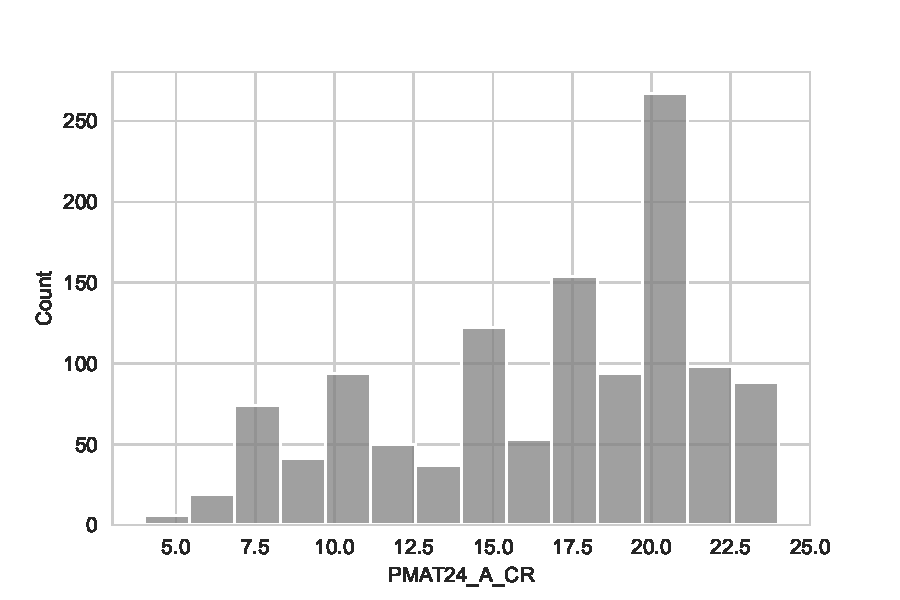
\includegraphics[width=0.36\paperwidth]{fig/hcp_iq_nonnorm_hist.pdf}
   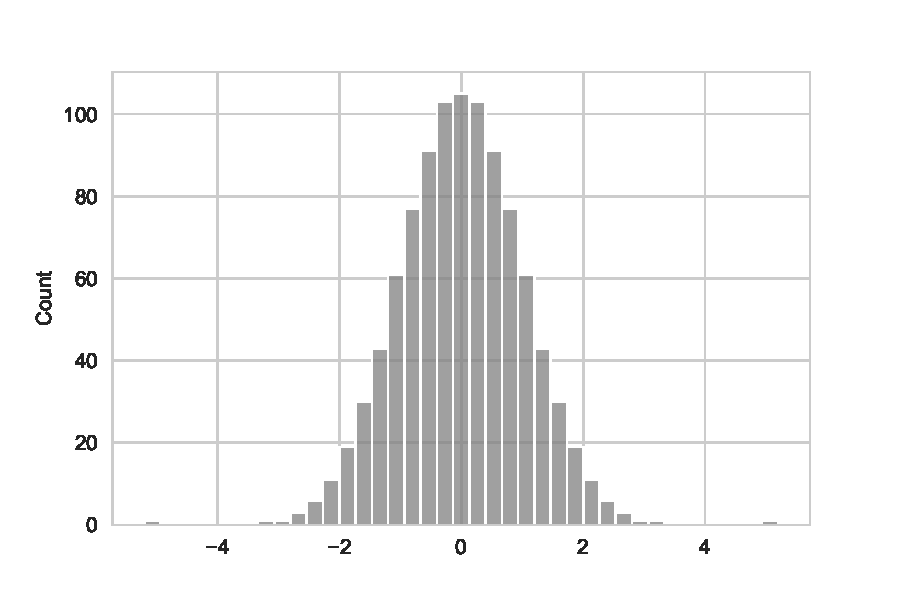
\includegraphics[width=0.36\paperwidth]{fig/hcp_iq_quanttrf_hist.pdf}
   }
  \caption{Histogram of fluid intelligence score in the HPC dataset, before (left) and after (right) quantile transformation.}
  \label{fig:hcp-hist}
\end{figure}

\begin{figure}[H]
  \centering
  \fbox{
   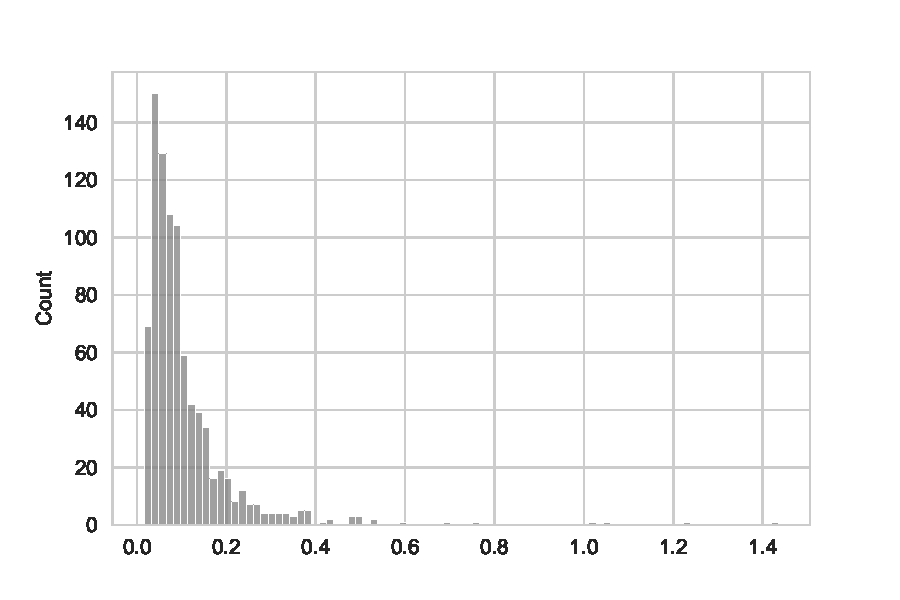
\includegraphics[width=0.36\paperwidth]{fig/abide_motion_hist.pdf}
   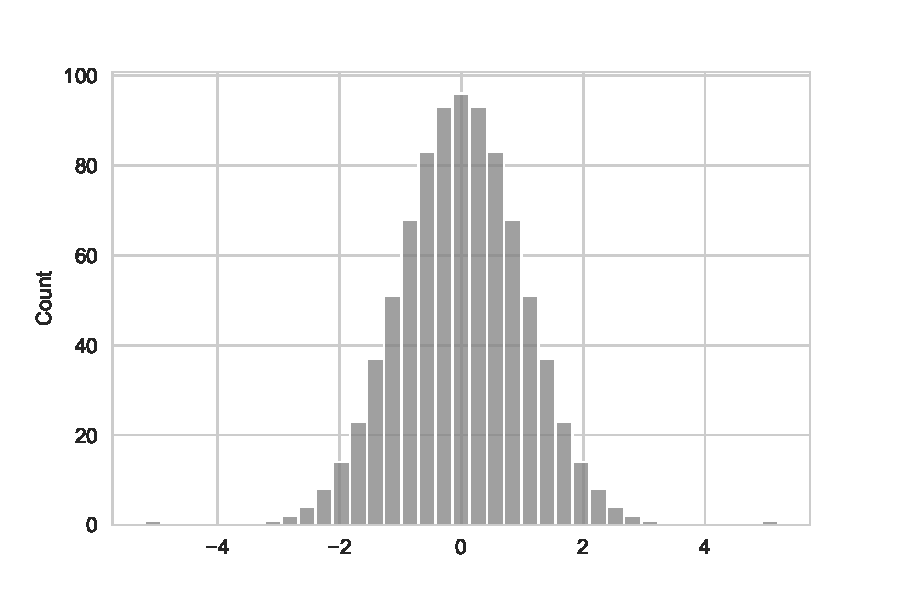
\includegraphics[width=0.36\paperwidth]{fig/abide_motion_quanttrf_hist.pdf}
   }
  \caption{Histogram of mean framewise displacement in the ABIDE dataset, before (left) and after (right) quantile transformation.}
  \label{fig:abide-hist}
\end{figure}

%TC:endignore

\end{document}
